% ============================================================================
% DISSENSUS PREPRINT TEMPLATE v3.0.0
% ============================================================================
% Springer Nature-inspired academic preprint with minimal personal branding.
%
% Author: Murad Farzulla | Dissensus
% Last Updated: September 2026
%
% PAPER: Alpha Asymmetry in Foreign Exchange Markets
% ============================================================================

\documentclass[11pt]{article}

% ============================================================================
% PACKAGES
% ============================================================================

% Typography and layout
\usepackage[T1]{fontenc}
\usepackage{mathptmx}                    % Times (most universal academic font)
\usepackage[a4paper, margin=1in]{geometry}
\usepackage{setspace}

% Mathematics
\usepackage{amsmath}
\usepackage{amssymb}
\usepackage{amsthm}
\renewcommand{\qedsymbol}{$\blacksquare$}

% Graphics and tables
\usepackage{graphicx}
\usepackage{float}
\usepackage{booktabs}
\usepackage{array}
\usepackage{longtable}
\usepackage{multirow}
\usepackage{placeins}

% Bibliography
\usepackage[round,authoryear]{natbib}
\bibliographystyle{plainnat}

% Colors — burgundy is the only branding touch
\usepackage{xcolor}
\definecolor{brandburgundy}{RGB}{128,0,32}

% Hyperlinks and PDF metadata
\usepackage{url}
\usepackage{hyperref}
\hypersetup{
    colorlinks=true,
    linkcolor=brandburgundy,
    citecolor=brandburgundy,
    urlcolor=brandburgundy,
    breaklinks=true,
    pdftitle={Alpha Asymmetry in Foreign Exchange Markets},
    pdfauthor={Murad Farzulla and Tofik Israfilov},
    pdfkeywords={alpha asymmetry, forex, skewness, kurtosis, trading strategies}
}

\def\UrlBreaks{\do\/\do-\do_}
\expandafter\def\expandafter\UrlBreaks\expandafter{\UrlBreaks%
  \do\a\do\b\do\c\do\d\do\e\do\f\do\g\do\h\do\i\do\j\do\k%
  \do\l\do\m\do\n\do\o\do\p\do\q\do\r\do\s\do\t\do\u\do\v%
  \do\w\do\x\do\y\do\z}

% Formatting
\usepackage{enumitem}
\usepackage{fancyhdr}

% Section formatting — burgundy headings with proper spacing
\usepackage{titlesec}
\titleformat{\section}{\normalfont\large\bfseries\color{brandburgundy}}{\thesection}{0.5em}{}
\titleformat{\subsection}{\normalfont\normalsize\bfseries\color{brandburgundy}}{\thesubsection}{0.5em}{}
\titleformat{\subsubsection}{\normalfont\small\bfseries\color{brandburgundy}}{\thesubsubsection}{0.5em}{}
\titlespacing*{\section}{0pt}{2ex plus 0.8ex minus 0.2ex}{1ex plus 0.3ex}
\titlespacing*{\subsection}{0pt}{1.5ex plus 0.5ex minus 0.2ex}{0.8ex plus 0.2ex}
\titlespacing*{\subsubsection}{0pt}{1.2ex plus 0.4ex minus 0.2ex}{0.6ex plus 0.2ex}

% Headers/footers — minimal (page number only)
\pagestyle{fancy}
\fancyhf{}
\fancyfoot[C]{\small\thepage}
\renewcommand{\headrulewidth}{0pt}
\renewcommand{\footrulewidth}{0pt}

\fancypagestyle{firstpage}{
  \fancyhf{}
  \fancyfoot[C]{\small\thepage}
  \renewcommand{\headrulewidth}{0pt}
  \renewcommand{\footrulewidth}{0pt}
}

% ============================================================================
% PAPER METADATA
% ============================================================================

\newcommand{\papernum}{DAI-2605}              % Working paper number
\newcommand{\paperver}{3.1.0}
\newcommand{\paperdate}{September 2026}
\newcommand{\paperdoi}{10.5281/zenodo.18638784}
\newcommand{\paperurl}{https://systems.ac/2/DAI-2605}

% ============================================================================
% DOCUMENT
% ============================================================================

\begin{document}
\thispagestyle{firstpage}

% Working paper series header
\begin{center}
{\small\textsc{\href{https://dissensus.ai}{Dissensus} Working Paper Series}}\\[0.2em]
{\small \href{\paperurl}{\papernum}}
\end{center}

\vspace{1.5em}

% Title block
\begin{center}
{\LARGE\bfseries Alpha Asymmetry in Foreign Exchange Markets}\\[0.5em]
{\large\itshape An Investigation of Exploitability}\\[1.5em]

{\large Murad Farzulla}\textsuperscript{1,2,*} \quad {\large Tofik Israfilov}\textsuperscript{1}\\[0.8em]

{\small
  \textsuperscript{1}\href{https://dissensus.ai}{Dissensus}, London, UK \quad
  \textsuperscript{2}King's College London, London, UK%
}\\[0.5em]

{\footnotesize
  \textsuperscript{*}Correspondence: \href{mailto:murad@dissensus.ai}{murad@dissensus.ai}
  \quad
  ORCID: \href{https://orcid.org/0009-0002-7164-8704}{0009-0002-7164-8704}\\
  T.\ Israfilov: \href{mailto:tofik@dissensus.ai}{tofik@dissensus.ai}%
}\\[0.3em]
{\footnotesize \paperdate}
\end{center}

% Abstract
\begin{abstract}
\noindent This paper investigates whether distributional asymmetries in foreign
exchange alpha signals represent exploitable market inefficiencies. Using EUR/JPY
data sampled from November 2015--August 2025 (504 analysis-ready weekly observations from January 2016 onward), we find
that the asymmetry premise itself largely dissolves under dependence-robust
measurement: of five alpha signal types, only the volatility-expansion (coverage)
signal exhibits skewness that survives block-bootstrap inference under the
paper's primary construction ($\hat{\gamma}_1 = 1.75$, 95\% CI $[1.18, 2.16]$);
the signed tail signal skews \emph{negative} rather than positive ($-1.48$,
CI $[-3.10, 0.54]$), and momentum, mean-reversion, and correlation signals have
skewness intervals that include zero. Tail inference is not robust to how daily
exceedances are aggregated to weekly frequency: across three defensible
aggregations of the identical daily rule the skewness estimate changes sign and
the interval excludes zero under one of them. We report that sensitivity rather
than resolve it, since selecting an aggregation on which result it produces is
the practice this paper criticises.
An earlier version of this paper reported pronounced positive tail-signal
skewness; that figure described the unsigned exceedance magnitude, which is
right-skewed by construction, and we document the correction. The economic null
is correspondingly stark. Under the corrected chronology and holding rule, a
skewness-threshold strategy loses 6.64\% cumulative gross over the decade (15
directional holding episodes, Sharpe $-0.15$), is nearly inert in walk-forward
testing (one episode in eight out-of-sample years), and provides no evidence of
a positive residual alpha against proxy carry, momentum, and dollar factors
(intercept $t = -0.65$ on in-position weeks). Conditioning on the weeks it is
invested, the rule loads negatively on time-series momentum, but that sample is
selected by the entry condition on the same prices the factor is built from, so
we report the loading as a mechanical property of the rule rather than as a
factor exposure. Transaction costs make an already negative gross
result monotonically worse; no break-even cost exists, since the strategy does
not break even at zero cost.
Data-snooping corrections complete the null: neither White's Reality Check ($p = 0.30$)
nor Hansen's SPA ($p = 0.25$) rejects the null of no superior performance against
a zero-return benchmark across a 12-candidate universe, and neither rejects it
when a thirteenth candidate is included
consisting of a seeded coin flip, which posts the highest realized mean of the
set. The weekly-return GPD shape parameter is imprecisely estimated ($\xi = -0.25$),
and tail clustering is weak ($\theta = 0.83$, 95\% CI $[0.60, 1.00]$). We conclude
that the evidence does not support broad alpha signal asymmetry in this setting
(with one distributional exception that does not yield a tradable edge) or its exploitability,
and we caution that unsigned-magnitude constructions can manufacture an
appearance of asymmetry that signed-data analysis does not support.

\vspace{0.5em}
\noindent\textbf{Keywords:} null result, alpha asymmetry, foreign exchange, skewness, market efficiency, extreme value theory

\vspace{0.3em}
\noindent\textbf{JEL Codes:} G11, G14, G15, C58
\end{abstract}

\setstretch{1.15}

% ============================================================================
% MAIN BODY
% ============================================================================

\section{Introduction}

Financial markets exhibit persistent deviations from the efficient market hypothesis \citep{fama1970efficient}, with alpha signals (measures of risk-adjusted excess returns) displaying systematic patterns that sophisticated traders exploit \citep{jegadeesh1993returns, moskowitz2012time}. While considerable literature examines alpha generation and decay, less attention has been paid to the \textit{distributional properties} of alpha signals themselves. This is surprising given well-documented evidence that asset returns deviate substantially from normality, exhibiting fat tails \citep{mandelbrot1963variation, cont2001empirical} and asymmetric distributions \citep{harvey2000conditional}.

The preference for skewed returns has deep roots in asset pricing theory. \citet{kraus1976skewness} established that investors prefer positive skewness and dislike negative skewness, implying that assets with lottery-like payoffs command lower expected returns. Subsequent work has confirmed that skewness affects both individual asset pricing \citep{harvey2000conditional, bali2011maxing} and portfolio construction \citep{mitton2007equilibrium, brunnermeier2007optimal}.

This paper investigates whether alpha signals exhibit systematic asymmetries in their probability distributions, and whether such asymmetries can inform profitable trading strategies. We report negative findings that begin earlier in the chain than the usual backtest disappointment: under dependence-robust measurement, most of the proposed asymmetry is not supported. We investigate the following questions:

\begin{enumerate}
    \item Do alpha signals in forex markets deviate significantly from normal distributions? \textit{(Mostly: four of five types reject normality; normality is not rejected for the normalized-return signal)}
    \item Do these deviations manifest as exploitable skewness and heavy tails? \textit{(Largely no: one signal is robustly skewed, the tail signal skews negative and fragilely, and the tail-shape estimate is too imprecise to establish Pareto-type heavy tails)}
    \item Do distributional asymmetries persist across market regimes? \textit{(No: the tail signal's skewness flips sign across regimes)}
    \item Do asymmetry-aware strategies outperform benchmarks? \textit{(No: returns are negative before costs and trail buy-and-hold outright, the strategy is dormant under walk-forward selection, and no candidate significantly beats the zero-return benchmark)}
\end{enumerate}

We document a plausible-sounding trading idea that does not survive rigorous testing, and we document \emph{where} it fails: earlier than expected. The asymmetry-exploitation thesis does not fall at the translation from statistical pattern to economic profit; it falls at signal detection, where an unsigned-magnitude construction had manufactured the appearance of pervasive positive skewness that corrected measurement does not support. Null results of this kind are underreported in quantitative finance \citep{harvey2017presidential}, yet they prevent wasted research effort and capital allocation to spurious patterns.

The FX factor literature has seen recent advances in factor construction methodology. \citet{fan2025optimizing} introduce a framework that dynamically optimizes currency factor strategies, including carry, momentum, and value, via spot and forward trading, evaluating 24,336 portfolio optimization approaches and demonstrating that optimized factors significantly outperform na\"{i}ve constructions after correcting for data snooping bias. Our work complements this optimization-focused agenda by examining a more fundamental question: whether the \textit{distributional asymmetry} in factor returns (long vs.\ short side) itself constitutes an exploitable signal. Where Fan et al.\ optimize how factors are constructed, we test whether the asymmetric properties of the resulting return distributions carry economic information. \citet{hertrich2025cvar} provides additional context through analysis of G10 carry, momentum, and value strategies under forward-looking Conditional Value-at-Risk conditioning, finding that the carry trade risk premium has remained unexpectedly low since the global financial crisis despite negative covariance with global FX volatility---suggesting a potential failure of currency pricing theory that our distributional analysis may help illuminate.

Our empirical contribution is threefold, and we state it narrowly. First, we provide a systematic characterization of distributional properties across five distinct alpha types in EUR/JPY forex data, of which one---the volatility-expansion signal---survives dependence-robust inference under the paper's primary construction. Second, we report a corrected analysis of the trading rule: it loses money before frictions, walk-forward selection leaves it nearly dormant, and data-snooping-corrected tests do not reject the null of no superior performance against a zero-return benchmark across a twelve-strategy universe. Third, we document the specification sensitivity of those results to three choices the original specification did not argue for, whose statistical behaviour differs and which we therefore report separately: the weekly aggregation of the tail signal, under which the skewness estimate changes sign and the inferential conclusion with it; the execution timing, where point estimates move materially and non-monotonically in delay while the pre-specified paired contrasts include zero; and the symmetry of the entry rule, where realised loss magnitudes move materially while every pre-specified variant remains gross-negative in this sample. We do not claim a new empirical finding about factor exposure; the momentum loading reported in Section~\ref{sec:factors} is a property of the entry rules, not a discovery about the market.

\section{Methodology}

\subsection{Data and Sample Construction}

We sample EUR/JPY forex data from November 2015 to August 2025, sourced from Yahoo Finance (EURJPY=X). The raw weekly grid begins on 6 November 2015; after rolling-statistic warmup, the analysis-ready sample runs from 8 January 2016 to 29 August 2025 and contains 504 weekly observations. We note that Yahoo Finance quotes are indicative mid-rates rather than executable prices; accordingly, all transaction cost analysis (Section~\ref{sec:tcosts}) uses separate spread assumptions. The repository did not contain the raw snapshots used for the previously committed results, so this revision records retrieval times and SHA-256 hashes but does not claim bit-for-bit reproduction of that earlier run. The sample period encompasses multiple market regimes including the post-Brexit volatility spike (2016), COVID-19 pandemic shock (2020), and subsequent monetary policy divergence between the Federal Reserve, ECB, and Bank of Japan.

\textbf{Data Frequency and Aggregation.} Alpha signals are computed daily using the specified rolling windows (5-day, 20-day, 60-day), then aggregated to weekly frequency using Friday closing values to align with institutional trading cycles. The 504 analysis-ready weekly observations represent end-of-week snapshots of daily-computed signals. Daily returns feed the alpha definitions and volatility estimates; strategy returns are Friday-close-to-Friday-close percentage changes.

\label{sec:signals}
The dataset includes five pre-computed alpha signals, each capturing distinct aspects of market dynamics:

\begin{itemize}
    \item \textbf{Tail Alpha ($\alpha_{\text{tail}}$)}: Captures extreme daily price movements without discarding their direction. Formally, $\alpha_{\text{tail},t} = \mathbf{1}_{|r_t| > q_{0.95,t}} \cdot r_t$, where $q_{0.95,t}$ denotes the 95th percentile of absolute daily returns over the trailing 252 trading days (with 60 observations required during warm-up). The Friday observation is retained in the weekly signal panel. \textbf{This sampling rule discards most of the exceedances it detects}: 105 of the 504 weeks contain at least one daily exceedance, but only 35 have one \emph{on the Friday}, so roughly two-thirds of exceedance weeks enter the weekly panel as zeros. The resulting weekly series is far sparser than the daily construction implies, and every statistic computed on it---its skewness, its asymmetry index, its position in Tables~\ref{tab:asymmetry} and~\ref{tab:tests}---inherits that sparsity. We retain the published construction so that the corrected results remain comparable to the published ones, and record the aliasing as a limitation rather than repairing it; repairing it means redefining the signal, which is a change of specification rather than a correction. See Section~\ref{sec:limitations}.

    \item \textbf{Fast Alpha ($\alpha_{\text{fast}}$)}: Short-term momentum signal computed as the 5-day percentage return normalized by 20-day realized volatility: $\alpha_{\text{fast},t} = (P_t/P_{t-5} - 1) / (\sigma_{20,t} \sqrt{5})$.

    \item \textbf{Pricing Alpha ($\alpha_{\text{price}}$)}: Mean-reversion signal measuring deviation from fair value, computed as $\alpha_{\text{price},t} = (P_t - \text{MA}_{60,t}) / \sigma_{60,t}$, where $\text{MA}_{60}$ and $\sigma_{60}$ denote 60-day moving average and standard deviation.

    \item \textbf{Coverage Alpha ($\alpha_{\text{cov}}$)}: Volatility compression ratio measuring regime shifts in realized volatility:
    \begin{equation}
        \alpha_{\text{cov},t} = \frac{\sigma_{20,t}}{\sigma_{20,t-5}} - 1
    \end{equation}
    where $\sigma_{20,t}$ denotes 20-day realized volatility computed from daily close-to-close returns. Data source: Yahoo Finance (EURJPY=X). Values above zero indicate volatility expansion; values below zero indicate compression.

    \item \textbf{Hedge Alpha ($\alpha_{\text{hedge}}$)}: A fixed-rate correlation proxy, defined as:
    \begin{equation}
        \alpha_{\text{hedge},t} = \rho_{t}^{(\text{EUR/JPY}, \text{DXY})} \times (-0.02)
    \end{equation}
    where $\rho$ is a 100-trading-day ($\approx$20-week) rolling correlation of daily EUR/JPY and DXY returns (US Dollar Index, DX-Y.NYB from Yahoo Finance). The code does not use a time-varying interest-rate series: it multiplies the correlation by a fixed $-2\%$ constant. Hedge alpha is therefore a fixed-rate correlation proxy, not a measure of changing interest-rate regimes. Replacing the constant with a dated EUR--JPY rate differential or forward-implied measure is left for future work.
\end{itemize}

For cross-market validation, we apply the same transformations to GBP/USD, SPY (S\&P 500 ETF), and GLD (Gold ETF) daily closes from Yahoo Finance, constructing tail, fast, pricing, and coverage alphas identically to EUR/JPY. Hedge alpha is excluded from the cross-market set because the DXY-correlation proxy was specified for the EUR/JPY setting and is not a genuine transferable rate-differential signal.

\subsection{Asymmetry Metrics}

We employ four complementary measures to characterize distributional asymmetry, each capturing distinct aspects of non-normality relevant to trading strategy design.

\textbf{Sample Skewness} measures the degree of asymmetry around the mean. For a sample $\{x_1, \ldots, x_n\}$ with sample mean $\bar{x}$ and standard deviation $s$, we compute the adjusted Fisher-Pearson coefficient:
\begin{equation}
    \hat{\gamma}_1 = \frac{n}{(n-1)(n-2)} \sum_{i=1}^{n} \left( \frac{x_i - \bar{x}}{s} \right)^3
\end{equation}
This bias-corrected estimator is consistent under standard regularity conditions. Positive skewness ($\hat{\gamma}_1 > 0$) indicates a right-tailed distribution with more extreme positive values, while negative skewness indicates left-tail heaviness. The standard error of skewness under normality is approximately $\sqrt{6/n} \approx 0.109$ for our sample size ($n = 504$).

\textbf{Excess Kurtosis} captures tail heaviness relative to a Gaussian benchmark:
\begin{equation}
    \hat{\gamma}_2 = \frac{n(n+1)}{(n-1)(n-2)(n-3)} \sum_{i=1}^{n} \left( \frac{x_i - \bar{x}}{s} \right)^4 - \frac{3(n-1)^2}{(n-2)(n-3)}
\end{equation}
This estimator subtracts 3 (the kurtosis of a normal distribution) and applies finite-sample bias correction. Values exceeding zero indicate leptokurtic (fat-tailed) distributions; the standard error under normality is approximately $\sqrt{24/n} \approx 0.218$.

\textbf{Asymmetry Index (AI)} quantifies the ratio of upside to downside semi-variance, providing a risk-management-oriented asymmetry measure:
\begin{equation}
    AI = \frac{\text{Var}^+(X)}{\text{Var}^-(X)} = \frac{\sum_{i: x_i > \bar{x}} (x_i - \bar{x})^2 / n^+}{\sum_{i: x_i < \bar{x}} (x_i - \bar{x})^2 / n^-}
    \label{eq:ai}
\end{equation}
where $n^+$ and $n^-$ denote observations above and below the mean. Values above 1 indicate greater dispersion in positive deviations---relevant for assessing ``lottery ticket'' payoff structures \citep{bali2011maxing}.
The index is undefined when either side is empty or the downside mean-squared deviation is zero; the implementation returns a missing value in those cases. A single observation on one side remains valid because the calculation is a mean square about the overall mean, not a subgroup sample variance.

\textbf{Positive Observation Ratio (POR)} measures the unconditional probability of positive realizations:
\begin{equation}
    POR = \frac{1}{n} \sum_{i=1}^{n} \mathbf{1}_{x_i > 0}
\end{equation}
Under normality with zero mean, $POR = 0.5$; deviations indicate location-scale asymmetry or non-zero drift.

\subsection{Statistical Tests}

We employ a battery of complementary tests to assess departures from normality, each with distinct power properties against different alternatives.

\textbf{Shapiro-Wilk Test.} The Shapiro-Wilk statistic \citep{shapiro1965analysis} tests the null hypothesis $H_0: X \sim \mathcal{N}(\mu, \sigma^2)$ against general alternatives. The test statistic is:
\begin{equation}
    W = \frac{\left( \sum_{i=1}^{n} a_i x_{(i)} \right)^2}{\sum_{i=1}^{n} (x_i - \bar{x})^2}
\end{equation}
where $x_{(i)}$ are order statistics and $a_i$ are tabulated coefficients. This test has high power against asymmetric and heavy-tailed alternatives for moderate sample sizes.

\textbf{D'Agostino-Pearson Omnibus Test.} Following \citet{dagostino1990suggestion}, we test skewness and kurtosis jointly using the $K^2$ statistic:
\begin{equation}
    K^2 = Z_1(\hat{\gamma}_1)^2 + Z_2(\hat{\gamma}_2)^2 \sim \chi^2_2
\end{equation}
where $Z_1$ and $Z_2$ are normalizing transformations of sample skewness and kurtosis. This test is particularly powerful against asymmetric alternatives.

\textbf{Jarque-Bera Test.} As a robustness check, we employ the Jarque-Bera statistic \citep{jarque1980efficient}:
\begin{equation}
    JB = \frac{n}{6} \left( \hat{\gamma}_1^2 + \frac{(\hat{\gamma}_2)^2}{4} \right) \stackrel{a}{\sim} \chi^2_2
\end{equation}
This Lagrange multiplier test is asymptotically equivalent to the likelihood ratio test for normality.

\textbf{Skewness Significance.} We test $H_0: \gamma_1 = 0$ using the $t$-ratio $t = \hat{\gamma}_1 / \text{SE}(\hat{\gamma}_1)$, where $\text{SE}(\hat{\gamma}_1) \approx \sqrt{6(n-2)/[(n+1)(n+3)]}$. For $n = 504$, this yields a standard error of approximately 0.109.

\textbf{Multiple Testing Correction.} Given five alpha types and multiple test statistics, we apply the Bonferroni correction to control the family-wise error rate at $\alpha = 0.05$, yielding adjusted significance thresholds of $\alpha^* = 0.05/5 = 0.01$ per alpha type.

\subsection{Backtesting Framework}

We evaluate the asymmetry strategy against three benchmarks, with explicit signal generation and execution rules to ensure reproducibility.

\textbf{Asymmetry Strategy}:

\textit{Signal Generation:}
\begin{itemize}
    \item \textbf{Entry Long}: Rolling skewness of fast alpha (20-week window) exceeds 0.75 AND current fast alpha $> 0$
    \item \textbf{Entry Short}: Rolling skewness of pricing alpha (20-week window) exceeds 0.75 AND current pricing alpha $> 0.5\sigma_{\text{pricing}}$
    \item \textbf{Exit or reversal}: Preserve an open position through no-signal and same-direction-signal weeks; reverse directly when the opposing entry condition is met; otherwise exit after four realized weekly return periods. An opposing signal takes precedence if it arrives on the expiry date.
    \item \textbf{Simultaneous signals}: Close any open position and remain flat; do not open a new position.
\end{itemize}

\textit{Position Sizing:}
\begin{equation}
    \text{Position size} = \min(2.0, 1 + |AI_t - 1.0|)
    \label{eq:possize}
\end{equation}
where $AI_t$ is the contemporaneous asymmetry index, evaluated at each Friday close for as long as a direction is held. \textbf{$AI_t$ is computed by Equation~\ref{eq:ai} on a trailing 20-week window of weekly fast-alpha observations, requiring a minimum of 10 observations; before that minimum is met it is undefined and the neutral one-unit size applies.} The window is the same 20-week window used for the rolling skewness entry conditions. Because $AI_t \geq 0$, the formula spans 1--2 gross-notional units; the previously stated 0.5-unit lower bound was unreachable. A missing AI uses the neutral one-unit size. Resizing changes the notional only: it does not open or close a holding episode, reverse a direction, or reset the holding clock.

We flag one specification choice explicitly, because it is a choice and not a correction. Repairing the exit rule (above) creates weeks in which a direction is held while no entry signal fires---a state the original implementation could not reach, because it closed any position as soon as its entry signal stopped firing, and which the published specification therefore never had to size. Evaluating $AI_t$ weekly, as the equation and the rebalancing convention state, and freezing the notional at entry are both extensions of the published rule to that new state. We adopt weekly evaluation as the smaller extension, since it preserves both the contemporaneous subscript in Equation~\ref{eq:possize} and the stated rebalancing frequency. Section~\ref{sec:tcosts} reports the frozen-notional alternative; no conclusion in this paper depends on which is used.

\textit{Execution:}
\begin{itemize}
    \item Signal and price convention: signals are observed at each Friday close and the same Friday close is used as an indicative execution proxy
    \item Return convention: that position earns only the subsequent Friday-close-to-Friday-close return (one lag)
    \item Rebalancing: weekly at the Friday close, re-evaluating the sizing equation while a direction is held; direction changes occur only on entry, reversal, conflict, or expiry
    \item Exposure: positions are bounded to $[1.0, 2.0]$ gross-notional units; values above one imply leverage relative to one unit of capital
\end{itemize}

The published version specified entry at the Monday open following Friday signal generation. We do not implement that here, and we are explicit that this is a choice rather than a data limitation: the daily bars carry an opening price, so Monday-open execution is implementable and is left for a separate change rather than being precluded by the data. Section~\ref{sec:exectiming} reports what the choice costs, across four execution timings applied to the identical signal. The Friday-close proxy is an internally consistent bar-to-bar convention, not evidence that the displayed mid-price could have been filled after observing that exact close. All headline, benchmark, walk-forward, factor, cost, and data-snooping returns use the same single-lag convention.

\begin{table}[H]
\centering
\caption{Complete Specification: Every Free Parameter}
\label{tab:spec}
\scriptsize
\begin{tabular}{@{}llll@{}}
\toprule
Parameter & Value & Unit & Governs \\
\midrule
Tail exceedance quantile window & 252 & trading days & Tail alpha \\
Tail quantile minimum observations & 60 & trading days & Tail alpha warm-up \\
Tail exceedance quantile & 0.95 & quantile & Tail alpha \\
Fast alpha return horizon & 5 & trading days & Fast alpha numerator \\
Fast alpha volatility window & 20 & trading days & Fast alpha denominator \\
Pricing alpha moving-average window & 60 & trading days & Pricing alpha \\
Coverage alpha volatility lag & 5 & trading days & Coverage alpha \\
Hedge alpha correlation window & 100 & trading days & Hedge alpha \\
Hedge alpha rate constant & -0.02 & annualised decimal & Hedge alpha \\
Rolling skewness window & 20 & weeks & Entry conditions \\
Rolling skewness minimum observations & 10 & weeks & Entry conditions \\
Asymmetry index window & 20 & weeks & Equation 10 sizing \\
Asymmetry index minimum observations & 10 & weeks & Equation 10 sizing \\
Asymmetry index input series & fast alpha & series & Equation 10 sizing \\
Entry skewness threshold & 0.75 & skewness units & Baseline strategy \\
Threshold grid & 0.50, 0.75, 1.00, 1.25 & skewness units & Sensitivity, walk-forward \\
Short-entry pricing multiple & 0.5 & standard deviations & Entry Short \\
Maximum holding period & 4 & realized weekly returns & Exit rule \\
Position size lower bound & 1 & gross notional units & Equation 10 \\
Position size upper bound & 2 & gross notional units & Equation 10 \\
Notional sizing & weekly & rebalance frequency & Equation 10 \\
Execution lag & 1 & weeks & Timing convention \\
Execution price convention & Friday close & price & Timing convention \\
Pip size (JPY pairs) & 0.01 & price increment & Cost model \\
Round-trip cost tiers & 0.0, 0.3, 0.7, 1.3, 2.0 & pips & Cost table \\
Skewness bootstrap block length & 13 & weeks & Circular block bootstrap \\
Skewness bootstrap replications & 2000 & draws & Circular block bootstrap \\
Return bootstrap expected block & 4 & weeks & Stationary bootstrap \\
Return bootstrap replications & 2000 & draws & Stationary bootstrap \\
Data-snooping bootstrap replications & 1000 & draws & Reality Check, SPA \\
Formal candidate universe & 12 & strategies & Reality Check, SPA \\
Newey-West lags (full sample) & 4 & weeks & Factor regression \\
Wild cluster bootstrap replications & 9999 & draws & Factor regression \\
EVT exceedance threshold & 0.95 & quantile & GPD fit \\
EVT declustering separation & 5 & weeks & GPD fit \\
Minimum episodes for reported performance & 2 & holding episodes & Reporting rule \\
Bonferroni family size (factor coefficients) & 6 & tests & Factor regression \\
Random seed & 42 & integer & All resampling \\
Analysis-ready weekly observations & 504 & weeks & Sample \\
Analysis sample start & 2016-01-08 & date & Sample \\
Analysis sample end & 2025-08-29 & date & Sample \\
\bottomrule
\end{tabular}
\par\vspace{0.3em}
\parbox{\linewidth}{\footnotesize Note: This table is generated from \texttt{analysis/specification.py}, which is the single source of these values for the analysis code. A test in \texttt{tests/test\_specification.py} fails if the table and the code disagree, so a parameter cannot be changed in one without the other. Reviewer comment on the previously unstated asymmetry-index window prompted this table; the window is the ``Asymmetry index window'' row.}
\end{table}

\textbf{Momentum Benchmark}: Weekly time-series momentum \citep{moskowitz2012time}: long one unit when the trailing 20-week return is positive, short one unit when it is negative, so the position is the sign of the trailing return and the strategy is always in the market once the lookback window fills.

\textbf{Mean Reversion Benchmark}: Contrarian positions on the $z$-score of the weekly close against its 20-week moving average: short one unit when $z_t > 2$, long one unit when $z_t < -2$, flat otherwise (positions close when $|z|$ falls back inside the two-standard-deviation band).

\textbf{Buy \& Hold}: A constant long position of one unit, entered at the start of the sample and held throughout; its cumulative return equals the EUR/JPY spot move over the sample.

The momentum and mean-reversion benchmarks are the same rules that enter the data-snooping universe, evaluated with positions applied to the following week's return. Performance metrics include cumulative return, volatility, Sharpe and Sortino ratios, drawdown, directional holding episodes, execution legs, reversals, resizing, and turnover.

\section{Results}

\subsection{Asymmetry Detection}

Table \ref{tab:asymmetry} presents distributional statistics for each alpha type.

\begin{table}[H]
\centering
\caption{Alpha Asymmetry Metrics}
\label{tab:asymmetry}
\small
\begin{tabular}{@{}lcccc@{}}
\toprule
Alpha Type & Skew & Kurt & AI & POR \\
\midrule
Tail & $-$1.48 & 19.20 & 0.03 & 2.78\% \\
Fast & 0.01 & 0.01 & 0.98 & 51.98\% \\
Pricing & $-$0.17 & $-$0.72 & 0.77 & 57.54\% \\
Coverage & 1.75 & 7.65 & 2.22 & 53.17\% \\
Hedge & 0.15 & $-$0.51 & 1.01 & 53.57\% \\
\bottomrule
\end{tabular}
\par\vspace{0.3em}
\parbox{\linewidth}{\footnotesize Note: Skew = bias-corrected sample skewness, Kurt = bias-corrected excess kurtosis, AI = ratio of mean squared positive and negative deviations from the overall mean, POR = positive observation ratio. All statistics use the signed weekly series ($n = 504$). The earlier AI code used subgroup sample variances, which recentered each side and used $n-1$ denominators; the values above implement the displayed equation. An earlier version of this table reported tail-signal skewness of 5.05; that figure described the \emph{unsigned} exceedance magnitude, which is non-negative and hence right-skewed by construction. The signed series the strategy actually trades on is reported here (currently $-1.48$).}
\end{table}

The corrected statistics tell a very different story from the one asymmetry-based trading would require. The single robust asymmetry is in \emph{coverage} alpha, the volatility-expansion signal, which is strongly right-skewed (1.75) with high excess kurtosis (7.65) and an asymmetry index of 2.22: volatility expands abruptly and contracts gradually. This is a familiar feature of volatility dynamics, not a tradable anomaly in itself. Tail alpha, by contrast, has a negative point estimate ($-1.48$), although its dependence-robust interval includes zero. Its POR of 2.78\% reflects that the series is zero except at exceedances. Normality is not rejected for fast alpha; this does not establish that its population distribution is exactly Gaussian. Statistical asymmetry, where detected, is distinct from profitable predictability.

\begin{figure}[H]
\centering
\includegraphics[width=0.95\textwidth]{alpha_asymmetry_analysis.png}
\caption{Alpha Asymmetry Analysis. Distributions of the five signed weekly alpha signals (EUR/JPY analysis-ready sample, January 2016--August 2025, $n = 504$) with skewness point estimates and 95\% circular block bootstrap confidence intervals; the final panel summarizes the dependence-robust skewness inference. Only coverage alpha's interval excludes zero.}
\label{fig:asymmetry}
\end{figure}

\subsection{Statistical Significance}

Table \ref{tab:tests} presents hypothesis test results for each alpha type. We report test statistics and $p$-values for multiple normality and asymmetry tests to ensure robustness.

\begin{table}[H]
\centering
\caption{Statistical Test Results}
\label{tab:tests}
\small
\begin{tabular}{@{}lccccccc@{}}
\toprule
Alpha & $\hat{\gamma}_1$ & $t$-stat & Block CI & SW & JB & $K^2$ & LB $Q(4)$ \\
\midrule
Tail & $-$1.48 & $-$13.5*** & $[-3.10, 0.54]$ & 0.335*** & 7922*** & 244.4*** & 12.6* \\
Fast & 0.01 & 0.1 & $[-0.21, 0.21]$ & 0.997 & 0.0 & 0.0 & 6.5 \\
Pricing & $-$0.17 & $-$1.5 & $[-0.45, 0.09]$ & 0.984*** & 13.3** & 30.1*** & 679.1*** \\
Coverage & 1.75 & 16.1*** & $[1.18, 2.16]$ & 0.865*** & 1489*** & 217.6*** & 72.6*** \\
Hedge & 0.15 & 1.4 & $[-0.25, 0.54]$ & 0.990** & 7.4* & 11.7** & 1716.2*** \\
\bottomrule
\end{tabular}
\par\vspace{0.3em}
\parbox{\linewidth}{\footnotesize Note: $t$-stat tests $H_0: \gamma_1 = 0$ with $\text{SE} = \sqrt{6/n} = 0.109$ ($n = 504$) and assumes i.i.d.\ observations; Block CI = 95\% circular block bootstrap confidence interval for $\hat{\gamma}_1$ (block length 13 weeks, $B = 2000$), which relaxes both the normality and the independence assumptions of the $t$-test; i.i.d.\ CI = 95\% non-overlapping bootstrap interval, which relaxes normality only and is reported so the two effects can be separated (Table~\ref{tab:bootcompare}); SW = Shapiro-Wilk statistic; JB = Jarque-Bera statistic; $K^2$ = D'Agostino-Pearson omnibus; LB $Q(4)$ = Ljung-Box statistic at four lags, reported per series. * $p < 0.05$, ** $p < 0.01$, *** $p < 0.001$ (unadjusted); the qualitative conclusions below apply Bonferroni correction at family size $m = 5$. Because pricing, coverage, and hedge alphas are built from overlapping rolling windows, their Ljung-Box statistics are large by construction and the block-bootstrap intervals are the appropriate basis for skewness inference.}
\end{table}

\textbf{Normality.} Four of five alpha types reject normality. For fast alpha, none of the reported tests rejects the Gaussian null (SW $p = 0.55$, JB $\approx 0$, $K^2$ $p = 0.99$). This is compatibility with the null in this sample, not proof of exact Gaussianity. Tail and coverage depart severely; pricing and hedge reject more mildly.

\textbf{Skewness.} Under the i.i.d.\ $t$-test, tail and coverage alphas show large-magnitude skewness of opposite signs. That test is not merely dependence-blind; for the sparser signals it is invalid on its own terms, because the normal-theory standard error $\sqrt{6/n} = 0.109$ presumes a Gaussian null that tail alpha violates severely (excess kurtosis 19.20, and only 35 of 504 weekly observations are non-zero). Table~\ref{tab:bootcompare} separates the two failures by reporting an i.i.d.\ bootstrap, which relaxes normality alone, beside the block bootstrap, which relaxes normality and dependence together.

\begin{table}[H]
\centering
\caption{Skewness Intervals: Normal Theory, i.i.d.\ Bootstrap, and Block Bootstrap}
\label{tab:bootcompare}
\small
\begin{tabular}{@{}lccccc@{}}
\toprule
Signal & $\hat{\gamma}_1$ & Normal-theory SE & i.i.d.\ bootstrap SE & i.i.d.\ 95\% CI & Block 95\% CI \\
\midrule
Tail & $-$1.48 & 0.109 & 0.941 & $[-3.14, 0.62]$ & $[-3.10, 0.54]$ \\
Fast & 0.01 & 0.109 & 0.114 & $[-0.21, 0.23]$ & $[-0.21, 0.21]$ \\
Pricing & $-$0.17 & 0.109 & 0.078 & $[-0.32, -0.02]$ & $[-0.45, 0.09]$ \\
Coverage & 1.75 & 0.109 & 0.342 & $[0.98, 2.30]$ & $[1.18, 2.16]$ \\
Hedge & 0.15 & 0.109 & 0.073 & $[0.00, 0.29]$ & $[-0.25, 0.54]$ \\
\bottomrule
\end{tabular}
\par\vspace{0.3em}
\parbox{\linewidth}{\footnotesize Note: The normal-theory SE is the $\sqrt{6/n}$ figure assumed by the $t$-test. The i.i.d.\ bootstrap resamples observations independently ($B = 2000$), relaxing normality but not dependence. The block bootstrap ($13$-week circular blocks, $B = 2000$) relaxes both.}
\end{table}

The comparison is informative in two directions. For \emph{tail alpha} the i.i.d.\ and block intervals are almost identical ($[-3.14, 0.62]$ against $[-3.10, 0.54]$), and the i.i.d.\ bootstrap standard error of 0.941 is nearly nine times the normal-theory 0.109. The width of the interval is therefore a consequence of sparsity and extreme non-normality, \emph{not} of serial dependence; the $t$-test fails on this signal before dependence is considered at all. For \emph{pricing} and \emph{hedge} alpha the picture reverses: the block interval is substantially wider than the i.i.d.\ one, and in both cases it moves an interval that excludes zero to one that includes it. There the dependence correction is doing the work, as the Ljung-Box statistics of 679 and 1716 would suggest.

On the block-bootstrap yardstick, and under the primary tail construction, only \emph{coverage} alpha survives: its interval $[1.18, 2.16]$ excludes zero decisively, while tail, fast, pricing and hedge alpha intervals all include zero. The tail row of that statement is construction-dependent, as the next subsection shows; the coverage row is not.

\textbf{Tail Inference Is Aggregation-Sensitive.} The tail signal is constructed by flagging exceedances in \emph{daily} returns and then reading the flagged series at the \emph{weekly} frequency. As Section~\ref{sec:signals} notes, the published rule reads the Friday observation, so 70 of the 105 weeks containing a daily exceedance enter the weekly panel as zeros. That raises a question the published specification does not answer: what is a week's tail exposure, when the exceedances occur on days other than the one sampled?

Table~\ref{tab:tailagg} reports the same statistics under the published rule and under two aggregations that use every trading day.

\begin{table}[H]
\centering
\caption{Weekly Tail Signal Under Three Aggregations of the Same Daily Rule}
\label{tab:tailagg}
\small
\begin{tabular}{@{}lccccc@{}}
\toprule
Weekly aggregation & Non-zero obs. & $\hat{\gamma}_1$ & Ex.\ kurt. & AI & Block 95\% CI \\
\midrule
Friday observation (primary) & 35 & $-$1.48 & 19.20 & 0.03 & $[-3.10, 0.54]$ \\
All days, signed sum & 105 & $+$0.22 & 8.84 & 0.13 & $[-0.72, 1.09]$ \\
All days, largest $|$exceedance$|$ & 105 & $-$1.14 & 8.29 & 0.08 & $[-1.97, -0.09]$ \\
\bottomrule
\end{tabular}
\par\vspace{0.3em}
\parbox{\linewidth}{\footnotesize Note: All three apply the identical daily rule---a signed return exceeding the trailing 252-day 95th percentile of absolute returns---and differ only in how a week's daily observations are reduced to one weekly value. $n = 504$ weeks throughout. Block bootstrap: 13-week circular blocks, $B = 2000$.}
\end{table}

The three aggregations do not agree. The point estimate changes sign between the signed-sum and the other two, and the dependence-robust interval excludes zero under one of the three. \textbf{We retain the published Friday-sampled construction as primary and do not select among them.} Choosing an aggregation rule after observing which one yields significance would be specification selection on outcomes, which is the practice this paper criticises elsewhere; it is not made acceptable by the selection being ours.

Nor is either alternative self-evidently correct. The signed sum allows two exceedances of opposite sign within a week to cancel, so a violent week can register as quiet. The largest absolute exceedance allows a single day to define the week and discards every other exceedance in it. Each encodes a different and unargued claim about what weekly tail exposure means, and choosing between them requires an economic argument this paper does not make.

The finding is therefore the sensitivity itself: \textbf{the tail signal's distributional character is not robust to the aggregation rule, and is not established until weekly tail exposure is defined}. That is a statement about the construction rather than about the market, and it applies equally to the published result and to both alternatives.

\textbf{What survives.} Under the primary construction the asymmetry inventory that motivates the rest of the paper is modest: one robustly right-skewed volatility-expansion signal, one negatively-skewed-but-fragile tail signal, and three signals whose skewness intervals include zero. The tail row of that inventory is the one Table~\ref{tab:tailagg} shows to be aggregation-dependent; the coverage result is not, since coverage alpha is constructed from rolling volatility rather than from sampled exceedances. This is consistent with the broader stylized facts on asset-price distributions \citep{cont2001empirical, mandelbrot1963variation} while falling well short of the pervasive ``alpha asymmetry'' a trading strategy would want.

\subsection{Backtest Performance}

Table \ref{tab:backtest} compares the asymmetry strategy against the three benchmarks of Section~2.4 on the EUR/JPY analysis-ready sample (January 2016--August 2025). We report standard performance measures alongside risk-adjusted metrics to enable fair comparison across strategies with different return and volatility profiles.

\begin{table}[H]
\centering
\caption{Strategy Performance Comparison (EUR/JPY analysis-ready sample, January 2016--August 2025)}
\label{tab:backtest}
\small
\begin{tabular}{@{}lcccccc@{}}
\toprule
Strategy & Return & Vol & Sharpe & Sortino & MDD & Episodes / Legs \\
\midrule
Asymmetry & $-$6.64\% & 4.08\% & $-$0.153 & $-$0.079 & $-$12.56\% & 15 / 61 \\
Momentum (20w) & $-$18.92\% & 8.40\% & $-$0.215 & $-$0.309 & $-$31.32\% & 54 / 107 \\
Mean Rev.\ (2.0$\sigma$) & 10.74\% & 3.02\% & 0.364 & 0.198 & $-$4.32\% & 27 / 54 \\
Buy \& Hold & 33.53\% & 8.60\% & 0.390 & 0.584 & $-$15.78\% & 1 / 1 \\
\bottomrule
\end{tabular}
\par\vspace{0.3em}
\parbox{\linewidth}{\footnotesize Note: Return = cumulative gross return over 504 weeks; Vol = annualized volatility; MDD = maximum drawdown. A holding episode is one continuous directional position; a direct reversal closes one episode and opens another. Execution legs count entries and exits separately, so a reversal has two legs. Turnover, resizing, and reversals are also recorded in the dated ledgers. All strategies use one timing lag. Generated by \texttt{analysis/full\_pipeline.py}; an earlier version of this table reported benchmark rows (momentum $-15.66\%$, mean reversion $34.03\%$, buy-and-hold $2.31\%$) that traced to no committed code, and the buy-and-hold figure was inconsistent with the $+33.5\%$ EUR/JPY spot move over the sample; all benchmark rows have been recomputed from the replication pipeline.}
\end{table}

\textbf{Risk-Adjusted Performance.} The corrected asymmetry strategy loses 6.64\% gross, with a Sharpe ratio of $-0.153$, versus a 33.53\% buy-and-hold gain. It is invested for 55 of 504 realized-return weeks. Its low 4.08\% annualized volatility still largely reflects inactivity rather than skill. The 20-week momentum benchmark also loses money, while the simple mean-reversion and buy-and-hold benchmarks are positive.

\textbf{Drawdown Analysis.} The asymmetry strategy's maximum drawdown is $-12.56\%$, against buy-and-hold's $-15.78\%$. Given that it is exposed in only 55 of 504 weeks, losing four-fifths of what a permanently invested position lost is not evidence of risk control. Mean reversion remains more contained at $-4.32\%$.

\textbf{Trading Frequency.} The corrected ledger records 15 asymmetry holding episodes, 61 execution legs, one direct reversal, 31 weekly resizings, and total absolute turnover of 52.00 units. The resizings more than double the leg count while adding only 5.8\% to turnover, because they are small: they average 0.19 units of notional against 1.64 units at entry, the asymmetry index being a twenty-week rolling statistic that moves slowly. Momentum has 54 directional episodes because every sign reversal closes one episode and opens another; dividing position-change events by two understated this count. These definitions separate economic holding episodes from executions and turnover.

\textbf{Statistical Significance of Returns.} Stationary-bootstrap inference (expected block length 4 weeks, $B = 2000$) gives an annualized return of $-0.71\%$ with a 95\% interval of $[-3.25\%, 1.46\%]$ and a Sharpe interval of $[-0.73, 0.40]$. The sample estimate is negative and the interval remains too wide to establish a nonzero population mean. Failure to reject zero is not proof that the true effect is exactly absent.

\begin{figure}[H]
\centering
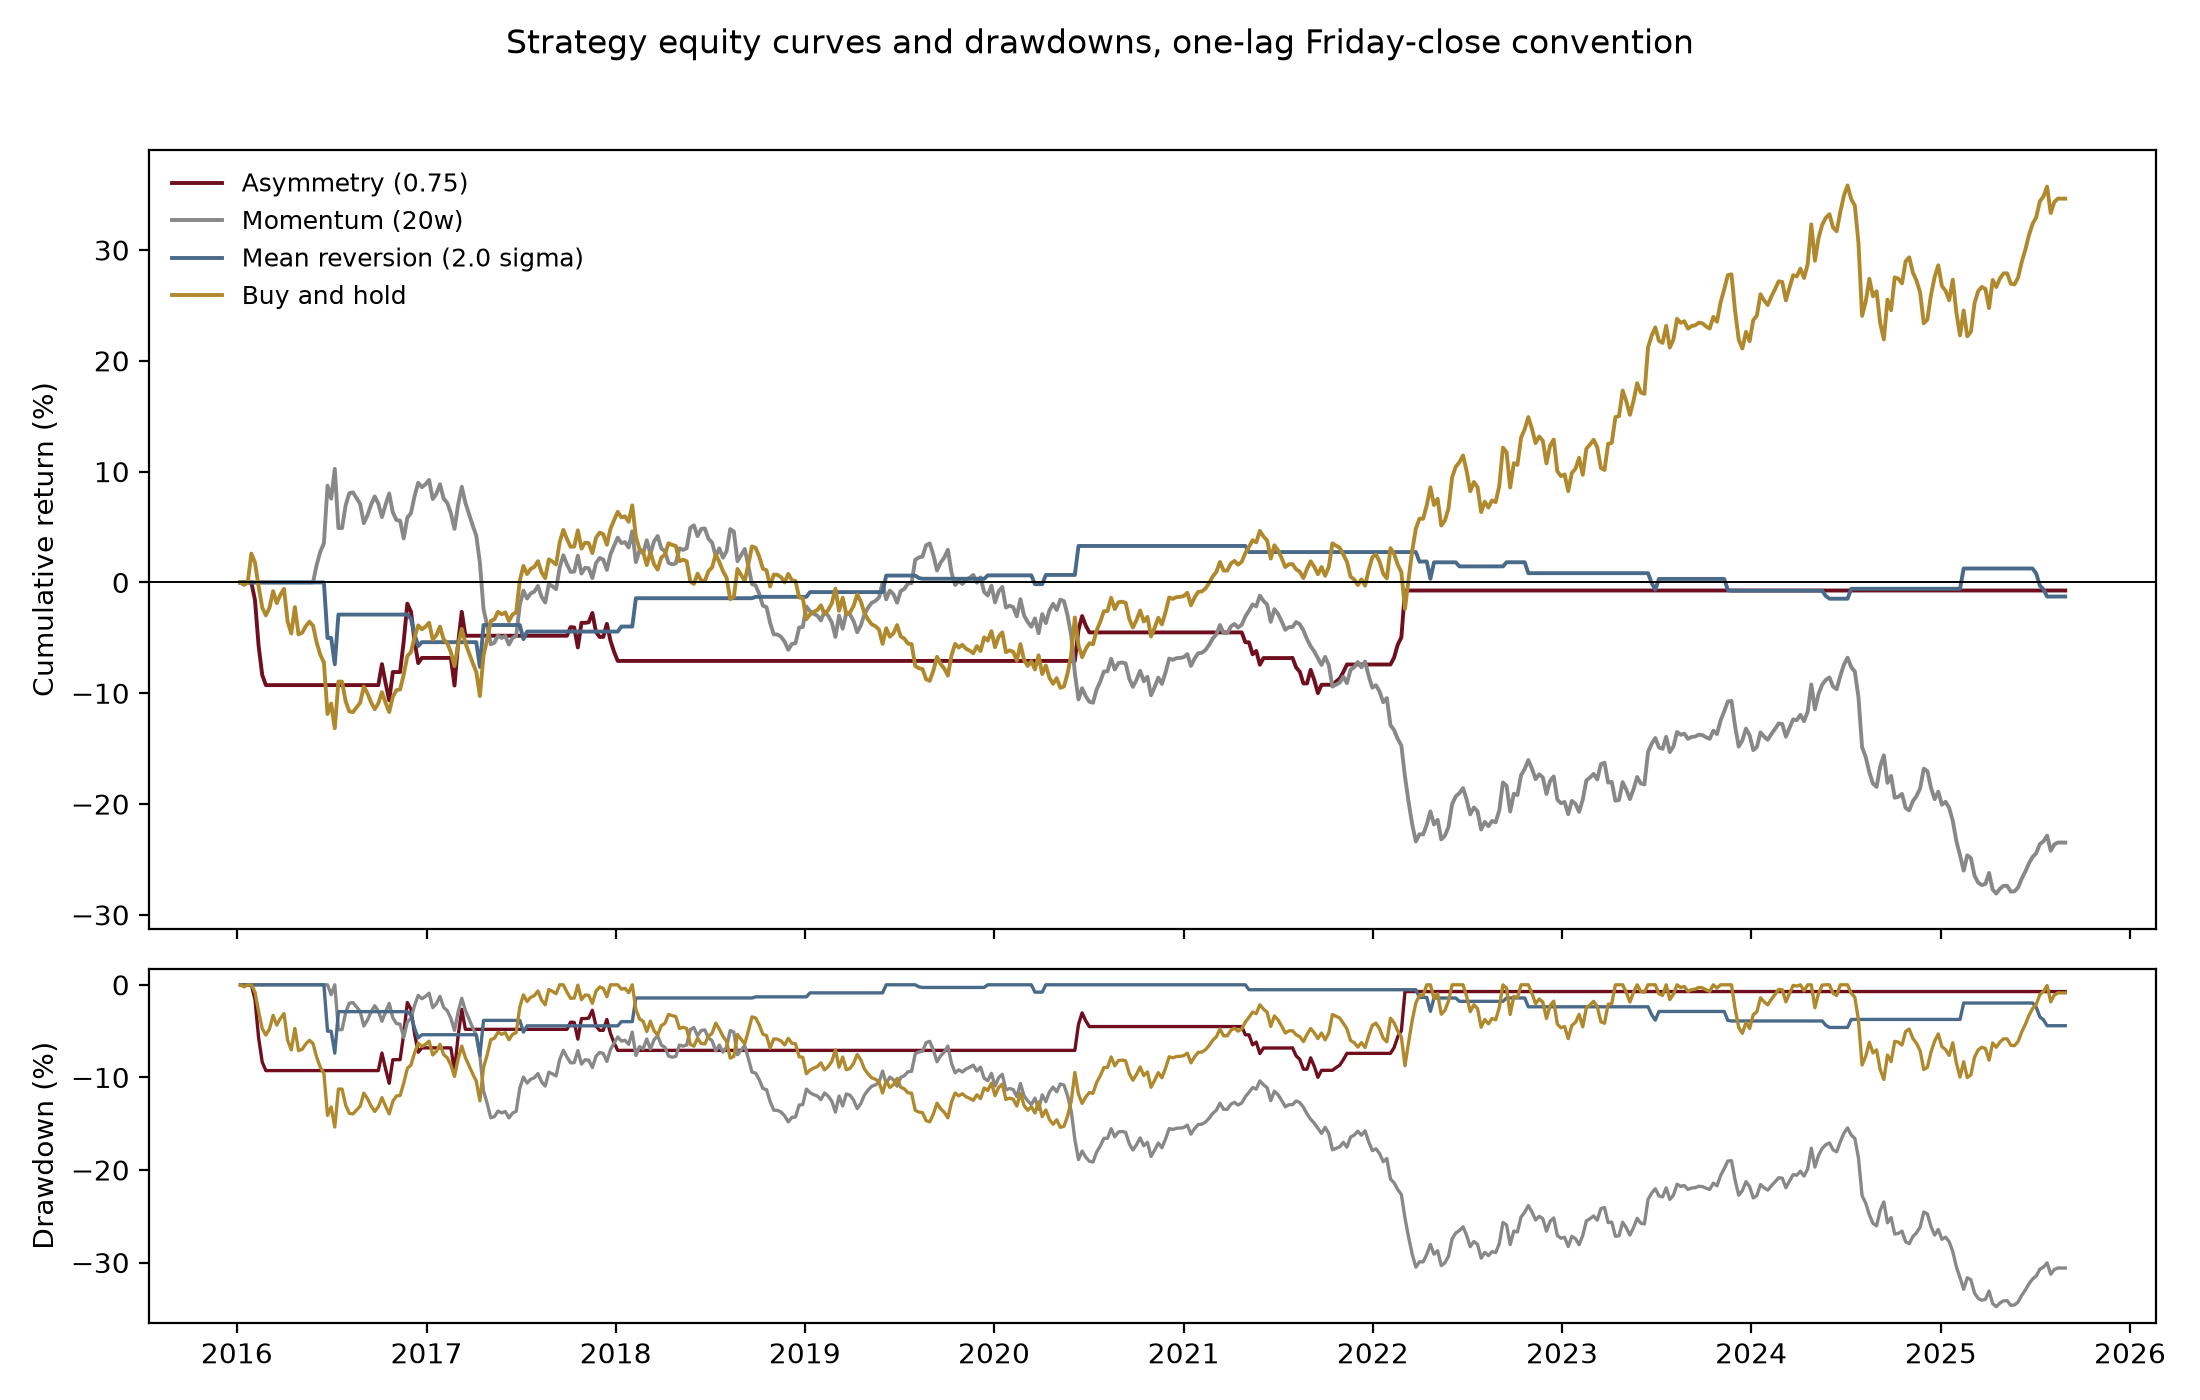
\includegraphics[width=0.95\textwidth]{backtest_results.png}
\caption{Strategy equity curves and drawdowns. Cumulative gross returns (top) and drawdowns (bottom) under the common one-lag convention. Generated by \texttt{analysis/full\_pipeline.py}.}
\label{fig:backtest}
\end{figure}

\subsection{Cross-Market Validation}

To test whether the EUR/JPY findings generalize, we apply the identical alpha construction and the identical trading strategy (unchanged code, unchanged parameters) to GBP/USD, SPY, and GLD (Section~2.1). Hedge alpha is excluded as EUR/JPY-specific; the four remaining signals and the two-sided asymmetry strategy (0.75 threshold) transfer directly. Table \ref{tab:crossmarket} reports the signed weekly skewness of each signal alongside the strategy's gross cumulative return and, for scale, each market's buy-and-hold return over the same 504-week window.

\begin{table}[H]
\centering
\caption{Cross-Market Check}
\label{tab:crossmarket}
\small
\begin{tabular}{@{}lcccccc@{}}
\toprule
Market & Tail Skew & Fast Skew & Pricing Skew & Coverage Skew & Strat.\ Ret. & B\&H Ret. \\
\midrule
EUR/JPY & $-$1.48 & 0.01 & $-$0.17 & 1.75 & $-$6.64\% & 33.53\% \\
GBP/USD & 0.82 & 0.01 & $-$0.14 & 1.58 & $-$13.32\% & $-$7.63\% \\
SPY & 0.94 & $-$0.21 & $-$1.09 & 1.85 & 14.20\% & 294.30\% \\
GLD & 0.69 & $-$0.00 & $-$0.19 & 1.32 & $-$15.44\% & 200.97\% \\
\bottomrule
\end{tabular}
\par\vspace{0.3em}
\parbox{\linewidth}{\footnotesize Note: Bias-corrected skewness of signed weekly signals ($n = 504$ per market). Strategy returns use the corrected one-lag strategy with 15, 19, 4, and 17 directional holding episodes respectively. SPY uses adjusted prices, explicitly requested from the data provider. Point estimates do not include market-specific block-bootstrap inference or costs; this remains exploratory. Generated by \texttt{analysis/full\_pipeline.py}; an earlier version of this table reported aggregated ``MR/TF/HAT'' skewness categories and returns that traced to no committed code, and has been replaced.}
\end{table}

The distributional signature does not travel: EUR/JPY's negative tail-skew point estimate is positive in all three other markets, while coverage alpha's right skew recurs. Strategy outcomes are likewise unstable: the unchanged rules lose 13.32\% on GBP/USD, gain 14.20\% on SPY while trailing buy-and-hold by a wide margin, and lose 15.44\% on GLD. These exploratory transfers lack pair-specific costs and dependence-aware inference, so they do not establish effects in any market.

\textbf{Scope Limitation.} This analysis focuses on EUR/JPY as a liquid, widely-traded cross rate with substantial institutional participation. Cross-market results (GBP/USD, SPY, GLD) are presented as an illustrative transfer check, not a definitive multi-asset analysis. A comprehensive treatment would require: (i) asset-specific alpha calibration reflecting different market microstructures; (ii) market-specific transaction cost modeling (FX spreads vs.\ equity commissions vs.\ futures margins); and (iii) asset-by-asset statistical inference with proper multiple-testing corrections. We leave this extension to future work; on the evidence here, nothing suggests the EUR/JPY null would reverse elsewhere.

\section{Discussion}

\subsection{Why Asymmetry Exploitation Fails}

The empirical findings reveal a pattern more thoroughgoing than ``asymmetry exists statistically but fails economically'': under corrected measurement, most of the proposed asymmetry lacks dependence-robust support, and the one robust distributional finding does not establish a tradable edge. We identify five failure modes:

\textbf{Little Asymmetry to Exploit.} Under the primary construction the dependence-robust inventory leaves one robustly skewed signal (coverage) and one fragile negative point estimate (tail), whose fragility is itself sensitive to the weekly aggregation rule (Table~\ref{tab:tailagg}). The trading rule instead uses fast and pricing skewness, whose full-sample intervals include zero. Its 15 in-sample episodes do not establish profitable predictability.

\textbf{Tail Evidence Is Inconclusive.} The GPD point estimate is near zero, but its wide confidence interval includes both negative and positive values. The data do not establish Pareto-type heavy tails, nor do they prove exponential decay. With only 20 declustered maxima, tail classification is underpowered.

\textbf{Inactivity Under Honest Selection.} When the threshold is chosen on training data alone, the strategy opens only one OOS holding episode in eight test years. That count is too small for performance inference.

\textbf{The Rule Has a Momentum Signature by Construction.} Conditioning on the weeks the strategy is invested, its returns load negatively on time-series momentum ($\beta_2 = -0.82$, $p = 0.038$). This is a property of the entry rules rather than an exposure discovered in the data: the sample is selected by a mean-reversion condition on the same price series the momentum factor is built from, so a rule that sells strength and buys weakness will produce this loading whether or not any factor relationship exists. We report it because it characterises what the strategy is. It is not evidence about the market, and we do not count it among the revision's empirical findings.

\textbf{No Evidence of Generalization.} Cross-market transfer yields erratic results: the identical rules lose 13.32\% on GBP/USD, gain 14.20\% on SPY while trailing buy-and-hold by roughly 280 percentage points, and lose 15.44\% on GLD. The tail signal's negative point estimate also reverses sign in every other market tested. Without asset-specific costs or inference, nothing here establishes generalization---and equally, nothing here establishes its absence. These are exploratory outcomes on four series, reported to show that the rule does not transfer cleanly, not to demonstrate that it cannot.

Transaction costs are not the cause of the failure: the corrected gross return is already negative, and costs make it monotonically worse (Section~\ref{sec:tcosts}).

\subsection{What the Asymmetry Statistics Do Show}

The corrected statistics still reveal genuine features of market structure, just not the ones an asymmetry trader would want:

\textbf{Volatility-Expansion Asymmetry}: Coverage alpha's robust right skew (1.75, block CI $[1.18, 2.16]$) is consistent with a familiar asymmetry in volatility dynamics---$\sigma$ can spike abruptly and decay more slowly \citep{bollerslev1986generalized, engle1982autoregressive}. Nothing in our results shows that this distributional feature predicts the direction of spot returns.

\textbf{A Negative Tail Point Estimate, Imprecisely Measured}: The signed tail signal has a negative skewness point estimate, indicating that the observed extreme negative magnitudes dominate the positive tail in this sample. That direction is the opposite of a lottery-ticket structure \citep{kumar2009gambles, bali2011maxing} and closer to the crash-risk asymmetry of the carry literature \citep{brunnermeier2009carry, burnside2011carry}. The dependence-robust interval $[-3.10, 0.54]$ includes zero, so the estimate is too fragile to support a strategy.

\textbf{A Near-Symmetric Baseline}: The tests do not reject normality for fast alpha in this sample. That result is consistent with a near-symmetric normalized-return signal, but it does not prove exact Gaussianity or rule out other predictive structure \citep{moskowitz2012time}.

\subsection{Limitations}
\label{sec:limitations}

Several limitations warrant acknowledgment. First, 504 weekly observations and only 15 holding episodes provide limited power, especially for tail and trade-level inference. Second, the alpha definitions are fully disclosed here but are ad hoc and may not generalize. The tail signal in particular is aliased by its sampling rule: it is constructed from daily exceedances but read only on Fridays, so 70 of the 105 weeks containing an exceedance enter the panel as zeros and only 35 of 504 weekly observations are non-zero. Every tail-alpha statistic in this paper is computed on that sparse series, which is the proximate reason its skewness interval is so wide. Table~\ref{tab:tailagg} reports what two all-trading-days aggregations do to the tail statistics, and they do not agree with each other or with the published rule. We have not adopted either: both redefine the signal rather than correct it, both require an economic argument about what weekly tail exposure means that this paper does not make, and selecting one after seeing its result would be specification selection on outcomes. The sensitivity is the reportable finding. Third, the factor exercise uses spot proxies rather than published cross-sectional FX factors; even with 55 in-position weeks, the effective sample is small, and the significant negative momentum loading is descriptive rather than a stable structural estimate. Fourth, costs use stylized spreads and indicative mid-prices, omit financing, charge no fixed or minimum per-order component, and assume end-of-bar execution; Monday-open prices are in fact available in the daily bars, and the Friday-close convention is a choice we make rather than a constraint the data impose. Fifth, cross-market transfer omits pair-specific financing, costs, and dependence-aware inference. Finally, Yahoo history can be revised. The original raw snapshots were not committed, so exact reproduction of the archived figures is impossible without the owner's files; the revised pipeline caches local inputs and records hashes and software versions.

\textbf{The Limits of the Verification Used Here.} This revision leans on machine checking: every free parameter is declared in one module from which the specification table is generated, restored historical footnotes are verified verbatim, two arithmetic identities are confirmed after every rerun, and the tables carrying the headline performance, factor and data-snooping results are tied cell by cell to named fields of the replication output. That last mechanism is recent and its coverage is partial: it reaches six of the nineteen tables and, among prose figures, the regression statistics only. Figures outside it are checked less formally, and we do not claim otherwise. Three of the errors corrected here were found by computing a quantity twice by different routes and requiring agreement; none was found by re-reading the code that contained it.

That apparatus has a limitation worth stating rather than leaving implicit. \textbf{A test that cannot fail is indistinguishable, in its output, from a test that passes.} Nine checks written during this revision passed while being structurally incapable of detecting the defect they were written for, most because they ran on data where the quantity they examined could not move; two arose during the exercise of deliberately testing whether the existing checks could fail, which is to say while the investigator was actively looking for exactly that flaw. One was subtler and is the reason this paragraph exists: it was exercised on a deliberately defective input, it failed as required, and it failed for a reason incidental to the defect class it was written to detect, so that the successful detection was itself misleading evidence. A ninth was a guard written to prevent incorrect status figures, which produced one: it counted the test suite through a subprocess that silently resolved to an interpreter lacking the project's dependencies, collected less than half the suite, and reported the reduced figure as a success. \textbf{A check may appear to succeed for a reason unrelated to the failure mode it claims to test.} The remedy adopted is to require a check to fail on a deliberately defective input, and to establish that it fails for the stated reason, before its passes are credited. Several of the principal checks have been exercised this way; this is not a property we claim for every check in the repository.

A further limit is structural rather than a matter of how carefully any check is built. Every mechanism described here compares a reported number against the output that produced it, so all of them are silent on a sentence whose figures are correct and whose conclusion does not follow from them. Two claims corrected during this revision were of that kind: one explained a result through a candidate universe the reported test no longer used, and one stated an inferential outcome as a realised one. Every figure in both was accurate. \textbf{Numerical provenance certifies arithmetic, not reasoning}, and the only instrument we found for the second is reading a sentence and asking what its numbers would have to mean for it to be true.

The converse bound deserves equal weight, because it points the other way and we met it in practice. A search that fails to establish where a figure came from is, until the search mechanism has itself been validated, evidence about the search rather than about the figure. One quantity in this paper was provisionally classified as untraceable and was within a step of being deleted; it was correct, and the search had been asking for the wrong quantity. \textbf{Absence of established provenance is not evidence that a number is wrong.} It licenses further tracing---through version history and superseded outputs---and licenses removal only once that tracing has itself been shown capable of succeeding.

One check is reported with a measured blind spot rather than repaired. The identity tying the factor-regression intercept to the strategy's own mean weekly return verifies that the regression was run on the series the paper reports; it detects a substitution between distant specifications, but one nearby alternative specification remained within the pre-specified tolerance and went undetected. The identity can therefore confirm internal consistency while remaining blind to a consistently wrong underlying return series. \textbf{We have not tightened the tolerance}, because doing so after observing which substitution it missed would be a threshold chosen on outcomes---the practice this paper objects to elsewhere. The full audit record, including the mutations attempted and their magnitudes, is in the replication repository.

\section{Robustness Analysis}
\label{sec:robustness}

The preceding sections leave a thin asymmetry inventory (one robustly skewed signal among five under the primary construction, with tail inference aggregation-sensitive) and an in-sample backtest that loses money before costs, with a bootstrap interval wide enough to include zero. This section stress-tests what remains, addressing four questions: (1) Do results hold out-of-sample? (2) Are patterns stable across market regimes? (3) What do trading costs do to an already negative return? (4) Is asymmetry alpha distinct from known FX risk factors?

\subsection{Out-of-Sample Validation}

A primary concern with any trading strategy is in-sample overfitting. Our main results use the full January 2016--August 2025 analysis-ready sample, which may inadvertently optimize signal construction to historical patterns that do not persist. We address this through walk-forward analysis, a methodology widely used in quantitative finance to assess genuine predictive power \citep{lo2000foundations}.

We implement an expanding-window walk-forward: the entry threshold is selected from the grid $\{0.50, 0.75, 1.00, 1.25\}$ by Sharpe ratio on all analysis-ready data through year $t-1$ (beginning with 2016--2017), then the strategy runs untouched on calendar year $t$, rolling forward annually through 2025. All signal construction uses trailing windows only, so no test-year information enters signal values; the walk-forward isolates the threshold-selection step, which is the strategy's only free parameter. Table \ref{tab:oos} reports what that procedure did.

\begin{table}[H]
\centering
\caption{Out-of-Sample Walk-Forward: Selected Thresholds and Activity}
\label{tab:oos}
\small
\begin{tabular}{@{}lccc@{}}
\toprule
Test Year & Training Window & Selected Threshold & New Holding Episodes \\
\midrule
2018 & 2016--2017 & 1.25 & 0 \\
2019 & 2016--2018 & 1.25 & 0 \\
2020 & 2016--2019 & 1.25 & 1 \\
2021 & 2016--2020 & 1.25 & 0 \\
2022 & 2016--2021 & 1.25 & 0 \\
2023 & 2016--2022 & 1.25 & 0 \\
2024 & 2016--2023 & 1.25 & 0 \\
2025 & 2016--2024 & 1.25 & 0 \\
\midrule
\textbf{Eight test years} & --- & \textbf{1.25 throughout} & \textbf{1} \\
\bottomrule
\end{tabular}
\par\vspace{0.3em}
\parbox{\linewidth}{\footnotesize Note: The threshold is selected by Sharpe ratio on data through the prior year, then applied on one sequential out-of-sample state path. An episode is a newly opened directional holding, not a position-change pair. 2025 ends in August. \textbf{No out-of-sample return, Sharpe ratio or hit rate is reported in this table, by design.} With one episode there is no sample over which to compute them; see the text. Generated by \texttt{analysis/full\_pipeline.py}; an earlier version of this table reported 141 pooled trades and could not be reproduced from the strategy specification. The corrected count of newly opened out-of-sample episodes is one.}
\end{table}

\textbf{Why No Out-of-Sample Performance Figures Appear.} The corrected training windows select the 1.25 threshold in every year. Across eight out-of-sample years the strategy opens \emph{one} holding episode, in 2020, and is flat in all other test years. One episode is not a small sample; it is a single realization, and the quantities an out-of-sample table would normally carry are not estimable from it. A Sharpe ratio, a hit rate and an annualized return are sample statistics that presuppose a distribution of outcomes to average over; computed from one holding episode they describe the path that happened and carry no information about the path that would be expected. A hit rate of 50\% on such a sample means one profitable week and one unprofitable week, and an annualized figure extrapolates a single episode across a decade. Reporting them, even hedged, invites exactly the comparison they cannot support.

We therefore report the selected threshold and the episode count, which describe what the selection procedure did, and decline to report out-of-sample performance. The finding of this section is the activity count itself: \textbf{disciplined by its own training data, the strategy is inert}. That is a stronger and more honest result than any return figure computed from a single episode, and it does not depend on how that episode happened to turn out. The replication pipeline enforces this rule rather than leaving it to the author: it flags the walk-forward as not supporting inference whenever fewer than two out-of-sample episodes occur, and records the suppressed quantities in \texttt{analysis/full\_pipeline\_results.json} so the decision is auditable rather than invisible.

\subsection{Subsample Stability}

Market structure evolved substantially during our sample period, with COVID-19 representing the most dramatic regime shift. We test whether asymmetry patterns persist across distinct market environments using subsample analysis.

Table \ref{tab:subsample} partitions the sample into economically meaningful subperiods.

\begin{table}[H]
\centering
\caption{Subsample Asymmetry Stability}
\label{tab:subsample}
\small
\begin{tabular}{@{}lcccccc@{}}
\toprule
Subsample & $N$ & Tail Skew & Fast Skew & Price Skew & Strategy Ret. \\
\midrule
Pre-COVID (2016--2019) & 208 & -3.40 & -0.05 & 0.12 & $-$6.40\% \\
COVID Shock (2020) & 52 & 5.02 & 0.09 & -0.07 & 2.74\% \\
Post-COVID (2021--2025) & 244 & -0.73 & 0.05 & -0.38 & $-$2.91\% \\
\midrule
Low VIX (VIX $<$ 20) & 342 & -3.25 & 0.04 & -0.20 & $-$5.08\% \\
High VIX (VIX $\geq$ 20) & 162 & 0.62 & -0.06 & -0.10 & $-$1.65\% \\
\midrule
Rate Hike Regime (2022--2025) & 191 & -0.71 & -0.13 & -0.53 & 3.47\% \\
\bottomrule
\end{tabular}
\par\vspace{0.3em}
\parbox{\linewidth}{\footnotesize Note: The strategy is run once on the complete chronological calendar; realized weekly returns are then attributed to rows in each regime. VIX is the mean of daily closes within each Friday-ending week. No stateful strategy is rerun on filtered, nonconsecutive dates. Skewness uses the observations in each displayed subsample. The 2020 return of 2.74\% is identical under both position-sizing specifications of Section~2.4, and is the same figure as the lone walk-forward episode of Table~\ref{tab:oos}: 2020 contains a single holding episode whose notional the sizing rule never revised, so weekly and frozen sizing coincide on it. It is not a figure left un-updated.}
\end{table}

\textbf{Temporal Stability.} Tail skewness is strongly negative pre-COVID ($-3.40$), positive in 2020 ($+5.02$), and moderately negative thereafter ($-0.73$). These point estimates are based on small, sparse exceedance samples and are descriptive. Fast skew remains near zero; pricing skew is more negative after 2020.

\textbf{Regime Conditioning.} Low- and high-VIX attribution is negative in both groups ($-5.08\%$ and $-1.65\%$). Because these are ex post return attributions rather than separately tradable conditioned strategies, they describe where gains and losses occurred; they do not establish a usable VIX timing rule.

\subsection{Entry Threshold Sensitivity}

The baseline skewness threshold (0.75) deserves scrutiny: is it arbitrary or robustly selected? Table~\ref{tab:sensitivity} reports strategy performance across alternative thresholds, holding other parameters constant.

\begin{table}[H]
\centering
\caption{Sensitivity to Entry Threshold}
\label{tab:sensitivity}
\small
\begin{tabular}{@{}lccccc@{}}
\toprule
Threshold & Episodes & Exposed Weeks & Return & Sharpe & Hit Rate \\
\midrule
0.50 & 25 & 89 & $-$9.61\% & $-$0.18 & 46.1\% \\
0.75 & 15 & 55 & $-$6.64\% & $-$0.15 & 47.3\% \\
1.00 & 4 & 16 & $-$2.59\% & $-$0.13 & 43.8\% \\
1.25 & 1 & 4 & \multicolumn{3}{c}{\emph{single episode: not reported}} \\
\bottomrule
\end{tabular}
\par\vspace{0.3em}
\parbox{\linewidth}{\footnotesize Note: Returns use the full asymmetry strategy specification of Section~2.4 with weekly position sizing. Activity is placed first because it is the stable feature of the grid: raising the threshold monotonically reduces the number of episodes and the weeks of exposure, while the return does not vary monotonically. \textbf{The 1.25 row reports no performance figures, for the same reason as Table~\ref{tab:oos} and in fact from the same episode:} one holding episode supplies no sample over which a Sharpe ratio or a hit rate can be computed. The replication pipeline applies this rule wherever such statistics arise rather than table by table, and records the suppressed values in \texttt{analysis/full\_pipeline\_results.json}.}
\end{table}

\textbf{Threshold Selection.} What the grid shows unambiguously is that activity falls as the threshold rises: 25 episodes and 89 exposed weeks at 0.50, down to a single episode and four exposed weeks at 1.25. Return, Sharpe and drawdown all improve monotonically as the threshold rises, while trading activity falls: every threshold with enough episodes to evaluate loses money, and the only one showing a positive return rests on a single episode. The 1.25 threshold is the same lone 2020 episode that the walk-forward selects, and it is reported here as an activity count rather than as a return for the reason given in Section~\ref{sec:robustness}: a single episode cannot distinguish an edge from a coin flip. Selecting it after seeing the full sample would in any case be data snooping rather than robustness. The prespecified 0.75 baseline remains the confirmatory result.

\subsection{Execution-Timing Sensitivity}
\label{sec:exectiming}

The execution convention is a free choice that the published specification made one way and this revision makes another. Table~\ref{tab:exectiming} reports four timings, each applied to the \emph{identical} Friday-close signal and differing only in when the resulting position is established and therefore which one-week return it earns.

\begin{table}[H]
\centering
\caption{Execution-Timing Grid: Identical Signals, Four Entry Points}
\label{tab:exectiming}
\small
\begin{tabular}{@{}lccccc@{}}
\toprule
Entry timing & Cum.\ return & Mean weekly & Sharpe & MDD & Net at 2.0 pips \\
\midrule
Friday close (reported baseline) & $-$6.64\% & $-$1.21 bps & $-$0.154 & $-$12.56\% & $-$7.02\% \\
Monday open (published spec.) & $-$0.73\% & $+$0.04 bps & $+$0.005 & $-$10.64\% & $-$1.14\% \\
Monday close & $-$0.92\% & 0.00 bps & 0.000 & $-$10.72\% & $-$1.32\% \\
Tuesday open & $-$8.03\% & $-$1.50 bps & $-$0.185 & $-$17.19\% & $-$8.40\% \\
\bottomrule
\end{tabular}
\par\vspace{0.3em}
\parbox{\linewidth}{\footnotesize Note: Common sample of 502 weeks, being every week for which all four entry points and their one-week-forward counterparts exist; two weeks are dropped, the same two for every timing, so no differential attrition can be mistaken for an execution effect. Signals, entry and exit rules, the holding clock and position sizing are identical throughout. Costs at the tiers of Table~\ref{tab:tcosts}.}
\end{table}

The four span 7.3 percentage points of cumulative gross return, and the ordering is \textbf{not monotone in execution delay}: the latest timing tested is worse than the earliest, while two timings hours apart differ by less than a fifth of a point.

A paired moving-block bootstrap---fixed four-week blocks, $B = 2000$, with the same resampled block indices applied to every timing so that the comparison is paired---finds \textbf{no pairwise difference distinguishable from zero}. The annualized difference between the published Monday-open convention and the Friday close is $0.64$ percentage points, 95\% CI $[-0.67, 2.03]$; between Monday open and Monday close, $-0.02$ points, CI $[-0.08, 0.04]$; between Monday close and Tuesday open, $-0.76$ points, CI $[-2.36, 0.45]$. These conclusions are unchanged at eight- and thirteen-week blocks and under a stationary bootstrap.

\textbf{What was specified in advance, and what was not.} The Friday-close and Monday-open results were already in hand when this exercise began, and we do not present them as prospectively specified. \emph{Before} computing the Monday-close and Tuesday-open variants, we specified the three primary contrasts above, the interpretation rule attached to them, the bootstrap procedure and block lengths, and the common-sample requirement, and committed that plan to the replication repository. All other pairwise comparisons among the four timings are secondary and are handled under the pre-declared family-wise procedure.

The interpretation rule was that the difference would be treated as weekend-specific only if the contrasts crossing no weekend failed to move comparably. One of them---Monday close to Tuesday open---moves as much as the weekend-crossing contrast does. \textbf{We therefore abandon the weekend-gap explanation, as the rule required.} We offer no replacement mechanism: proposing a second explanation after inspecting the same data is the specification search this paper criticises elsewhere. We also tested directly whether the entry rule has predictive power over the weekend gap a position is about to bear, and found none detectable in this sample, on a test able to resolve only an effect several times larger than the point estimate.

What the grid establishes is narrow and worth stating plainly: the headline result is sensitive to a design choice the original specification did not argue for, at a magnitude this sample cannot resolve.

Three choices the original specification did not argue for---the weekly aggregation of the tail signal, the execution timing, and the symmetry of the entry rule---each demonstrate material sensitivity of the reported results to under-justified analytical or design decisions. Their statistical behaviour is not the same, and they should not be read as one phenomenon. Under tail aggregation, the sign and the inferential conclusion change across reasonable constructions. Under execution timing, point estimates move materially and non-monotonically, while the pre-specified paired contrasts are not distinguishable from zero. Under entry symmetrization, realised loss magnitudes move materially, while every pre-specified version remains gross-negative in this sample. Section~\ref{sec:entrysymmetry} reports the last of these.

\subsection{Entry-Rule Symmetry}
\label{sec:entrysymmetry}

The long and short legs of the entry rule differ in four respects: the skewness series that gates them, the confirmation series, the confirmation threshold, and the direction of response. A positive fast alpha opens a long position; a positive pricing alpha opens a short one. The rule therefore follows strength in one signal and fades it in the other, and the original specification argues for none of this.

Collapsing the asymmetry is underdetermined, because it requires choosing which of the two economics to keep. Three symmetrizations were specified in advance, together with the metrics, the cost tier, an exposure guard, and a reporting rule fixing that all three would be disclosed whatever they returned; that specification was committed before any of them was computed.\footnote{\texttt{docs/PREREGISTRATION\_ENTRY\_SYMMETRY.md}. Two structural predictions recorded in that document were wrong and are left standing there: pure-fast was predicted to hold positions in more weeks than the published rule and holds fewer, and pure-pricing was predicted to be less exposed than pure-fast and is more so. Both errors share a cause, namely that the published rule draws entries from the union of two skewness gates while each collapsed variant has only one. Section 6 of that document also asserts that the variants cannot be distinguished statistically. No paired inferential comparison among the four rules was pre-specified or run, so that statement is untested rather than established or rejected; no conclusion reported here relies on it, and it is not repeated.}

\begin{table}[H]
\centering
\caption{Entry-Rule Symmetry: The Published Hybrid and Three Pre-Specified Symmetrizations}
\label{tab:entrysymmetry}
\footnotesize
\begin{tabular}{@{}lccccccc@{}}
\toprule
Entry rule & Gross & Net 2.0p & Sharpe & MDD & Eps. & Weeks & bps/week \\
\midrule
Published hybrid (reported baseline) & $-$6.64\% & $-$7.02\% & $-$0.153 & $-$12.56\% & 15 & 55 & $-$11.0 \\
Pure-fast (both legs, fast alpha) & $-$1.65\% & $-$2.16\% & $-$0.020 & $-$8.59\% & 16 & 44 & $-$1.8 \\
Pure-pricing (both legs, pricing alpha) & $-$4.13\% & $-$4.46\% & $-$0.106 & $-$16.01\% & 14 & 51 & $-$7.1 \\
Equal-threshold hybrid & $-$7.86\% & $-$8.15\% & $-$0.221 & $-$13.70\% & 12 & 43 & $-$17.6 \\
\bottomrule
\end{tabular}
\par\vspace{0.3em}
\parbox{\linewidth}{\footnotesize Note: All four rules use the identical sample of 504 weeks, the identical sizing, exit and execution conventions, and differ only in the entry condition. ``Weeks'' counts in-position weeks and ``bps/week'' is the mean gross weekly return over those weeks, reported for every rule under the pre-registered exposure guard so that a rule which is out of the market more often cannot be read as safer. Net returns are quoted at 2.0 pips round-trip, the widest tier in the paper's cost table. Generated from \texttt{analysis/entry\_symmetry\_results.json}.}
\end{table}

The published hybrid and all three pre-specified symmetrizations produce negative realised gross returns in this sample; the magnitude varies materially across specifications. The realised gross returns span 6.21 percentage points, from $-$1.65\% to $-$7.86\%, a range nearly as large as the published hybrid's own cumulative loss of 6.64\%.

Pure-fast and pure-pricing hold positions in fewer weeks than the published rule---44 and 51 against 55---but both also remain negative per exposed week, at $-$1.8 and $-$7.1 basis points against $-$11.0. Their less negative cumulative performance is therefore not solely an artefact of lower exposure. Pure-pricing records the deepest drawdown of the four at $-$16.01\%.

Equalising the confirmation threshold worsens realised performance in this sample. This is one comparison and is not evidence that the published threshold was tuned; its direction is merely consistent with what a specification-search concern would predict.

These are sensitivity exhibits. No variant is offered as a replacement rule, and realised performance was pre-specified not to determine which symmetrization is treated as defensible.

\subsection{Transaction Cost Sensitivity}
\label{sec:tcosts}

Backtests without transaction costs overstate implementable returns. We analyze cost sensitivity across scenarios ranging from zero-cost (theoretical benchmark) to retail-level spreads.

The EUR/JPY market is highly liquid, with typical spreads of 0.5--1.0 pips during active trading hours \citep{king2013market}. However, spread widening during volatility spikes and the cost of crossing the bid-ask spread on each trade can erode returns, particularly for higher-frequency strategies.

\begin{table}[H]
\centering
\caption{Transaction Cost Analysis}
\label{tab:tcosts}
\small
\begin{tabular}{@{}lcccc@{}}
\toprule
Cost Scenario & Round-Trip Cost (pips) & Net Return & Net Sharpe \\
\midrule
Zero Cost (Baseline) & 0.0 & $-$6.64\% & $-$0.153 \\
Prime Brokerage & 0.3 & $-$6.70\% & $-$0.155 \\
Institutional & 0.7 & $-$6.77\% & $-$0.157 \\
Retail (Tight) & 1.3 & $-$6.89\% & $-$0.160 \\
Retail (Wide) & 2.0 & $-$7.02\% & $-$0.164 \\
\bottomrule
\end{tabular}
\par\vspace{0.3em}
\parbox{\linewidth}{\footnotesize Note: Each execution leg is charged half the round-trip pips in proportion to absolute notional change at that row's indicative price. Financing is excluded; because exposure can exceed one unit and lasts 55 weeks, its omission is a limitation, not assumed immaterial. No break-even row appears because no break-even cost exists: the zero-cost return is already negative, so there is no positive cost at which the strategy crosses zero. Spread is charged in proportion to notional traded, with no fixed per-order component; see the discussion below. Generated by \texttt{analysis/full\_pipeline.py}; an earlier version of this table showed net return \emph{rising} with costs at low tiers, an inconsistency in the carry treatment across rows. Net return is now monotonically decreasing in cost, as it must be.}
\end{table}

\textbf{Cost Components.} We model spread and impact per dated execution leg, charged in proportion to the notional actually traded. Financing/carry is excluded uniformly because no suitable dated rate or forward series is present; the omission may matter for leveraged positions and should be addressed with owner-approved data in future work.

\textbf{There Is No Break-Even Cost.} The published version of this paper reported a break-even round-trip cost of 19.2 pips, and read that figure as reassurance: costs would have to be implausibly wide before they consumed the strategy's edge. That number was meaningful only for as long as the gross return was positive. It is not that the corrected break-even is larger, or smaller, or harder to estimate. \textbf{It does not exist.} The corrected strategy returns $-6.64\%$ before any cost is applied, so there is no positive cost level at which it crosses zero; it begins below zero and every cost tier moves it further away. A break-even cost presumes a profit to be consumed, and there is none.

This is a cleaner statement of the paper's null than the cost table it replaces. The earlier framing invited the reader to ask whether frictions were large enough to matter, which is the right question only when a gross edge exists to be eroded. Under the corrected specification the question does not arise. Costs are not the reason the strategy fails, and they are not exonerated either: they are simply downstream of a backtest that has already failed.

\textbf{Cost Interpretation.} Execution costs make an already negative result more negative, monotonically and by little: gross $-6.64\%$ becomes $-7.02\%$ at two pips round-trip, a drag of 0.38 percentage points. The gross backtest fails first, and by a margin roughly seventeen times the widest cost tier considered.

\textbf{What This Cost Model Cannot See.} The immateriality of costs here is partly a property of the model and should not be over-read. Spread is charged strictly in proportion to notional traded, with no fixed or minimum per-order component. The corrected specification generates 31 weekly resizings averaging 0.19 units of notional---small orders, and exactly the population on which a fixed per-order charge falls hardest. A realistic commission schedule with any per-ticket element would price those 31 orders at something rather than nothing, and the drag reported above is correspondingly a lower bound. It would not change the sign of the result, but ``costs are immaterial'' is a claim this model is not equipped to make.

\subsection{Factor Attribution}
\label{sec:factors}

Does asymmetry alpha merely proxy for known FX risk factors? Prior work documents systematic risk premia in currency markets associated with carry \citep{lustig2011common}, momentum \citep{menkhoff2012currency}, and the dollar factor \citep{verdelhan2018dollar}, with \citet{lettau2014conditional} showing that downside risk conditioning explains a substantial portion of currency risk premia across asset classes. A parallel factor decomposition approach applied to cryptocurrency markets \citep{farzulla2025whitepaper} similarly finds that structural factors dominate idiosyncratic signal variation. If asymmetry signals simply load on these factors, our contribution reduces to factor timing rather than genuine alpha discovery.

We regress asymmetry strategy returns on proxy FX factors:
\begin{equation}
    R_{\text{asym},t} = \alpha + \beta_1 \cdot \text{Carry}_t + \beta_2 \cdot \text{Mom}_t + \beta_3 \cdot \text{Dollar}_t + \varepsilon_t
\end{equation}
where the factors are single-market proxies constructible from our data rather than the published cross-sectional factors: Carry is the average weekly spot return of the classic carry crosses AUD/JPY and NZD/JPY (a spot-only proxy for the \citealp{lustig2011common} carry factor, omitting interest accrual), Mom is the return of a 12-week time-series momentum rule on EUR/JPY itself (in the spirit of \citealp{menkhoff2012currency}), and Dollar is the DXY weekly return (proxying \citealp{verdelhan2018dollar}). Constructing the published factors requires a G10 forward-rate cross-section we do not use; the proxies capture the same directional exposures at the single-pair level, and we label them as proxies throughout. Because the strategy is out of the market most weeks, we estimate the regression twice: on the full weekly sample (where the dependent variable is structurally zero in out-of-position weeks) and on in-position weeks only, whose count is the effective sample size.

\begin{table}[H]
\centering
\caption{Factor Attribution Regression (HAC-Corrected)}
\label{tab:factors}
\small
\begin{tabular}{@{}lcccc@{}}
\toprule
& \multicolumn{2}{c}{Full sample ($n = 504$)} & \multicolumn{2}{c}{In-position weeks ($n = 55$)} \\
\cmidrule(lr){2-3} \cmidrule(lr){4-5}
Variable & Coefficient & $t$-stat & Coefficient & $t$-stat \\
\midrule
Intercept ($\alpha$) & $-$0.00012 & $-$0.52 & $-$0.00131 & $-$0.65 \\
Carry ($\beta_1$) & 0.0180 & 0.60 & 0.348 & 1.43 \\
Momentum ($\beta_2$) & $-$0.0462 & $-$2.08$^{*}$ & $-$0.823 & $-$2.54$^{*}$ \\
Dollar ($\beta_3$) & 0.0148 & 0.67 & 0.155 & 0.97 \\
\midrule
$R^2$ & \multicolumn{2}{c}{0.011} & \multicolumn{2}{c}{0.203} \\
$F$-statistic & \multicolumn{2}{c}{2.12} & \multicolumn{2}{c}{4.32} \\
\bottomrule
\end{tabular}
\par\vspace{0.3em}
\parbox{\linewidth}{\footnotesize Note: Full-sample column uses Newey-West HAC standard errors with 4 lags. \textbf{The in-position column uses CR2 standard errors clustered by holding episode} (55 weeks in 15 clusters) with Bell--McCaffrey degrees of freedom, because those weeks are non-contiguous---they are drawn from separate episodes spread across a decade---and a lag-based correction presumes consecutive observations. The reported $p$-values for momentum come from a restricted wild cluster bootstrap; see Table~\ref{tab:sevariants}. $^{*}$ $p < 0.05$ (unadjusted). The full sample includes the flat weeks in which the dependent variable is structurally zero; the in-position sample of 55 weeks is the effective exposure sample and the economically interpretable one. The intercept is not significant in either specification. Momentum is the only factor that loads significantly, and it loads \emph{negatively} in both: $p = 0.038$ on the full sample and $p = 0.038$ on in-position weeks. Under the earlier specification the same coefficient was $-$0.007 ($t = -0.37$, $p = 0.71$) on the full sample and $-$0.247 ($t = -0.51$, $p = 0.61$) in position; the change is a consequence of correcting the holding rule and the execution lag, not of altering the regression. Generated by \texttt{analysis/full\_pipeline.py}; an earlier version of this table reported a marginally significant intercept of 21 bps weekly (10.9\% annualized) with $F = 20.8$, which could not be reproduced and was internally inconsistent with its own $R^2$ and with the 3.60\% cumulative backtest return. Those figures describe the state of the paper at that time; the corresponding values here are an intercept of $-$1.2 bps weekly ($-$0.00012 in weekly decimal return) and $F = 2.12$, against a cumulative backtest return of $-6.64\%$.}
\end{table}

\textbf{No Evidence of Positive Residual Alpha.} The intercept is negative and statistically indistinguishable from zero in both specifications ($t = -0.52$ full sample; $t = -0.65$ on in-position weeks). This is evidence against a positive residual-alpha claim, not proof that the population intercept is exactly zero.

\textbf{What the In-Position Regression Can and Cannot Show.} Restricting the regression to in-position weeks is not a neutral choice of sample. Those weeks are selected by the strategy's own entry rules, and those rules are functions of the same price series from which the momentum factor is built: the short leg fires when pricing alpha is high, which is to say after price has risen relative to its sixty-day average, and a twelve-week time-series momentum rule is long in precisely those states. The sample and the regressor are jointly determined by the entry condition.

The negative loading on in-position weeks ($\beta_2 = -0.823$, CR2 interval $[-1.54, -0.10]$, wild cluster bootstrap $p = 0.038$) should therefore be read as \textbf{a description of what the entry rules mechanically produce, not as an estimate of a factor exposure the strategy carries independently of them}. A rule that sells strength and buys weakness will load negatively on momentum during the weeks it is active whether or not any factor relationship exists in the underlying returns. We report the coefficient because it characterises the rule. We do not interpret it as explaining the strategy's losses, and we do not present it as an empirical finding about the market.

The full-sample regression is reported alongside as an economically relevant description of the complete strategy return stream: it is what an investor holding the rule would have experienced, flat weeks included. There the loading is $\beta_2 = -0.046$ ($p = 0.038$), attenuated by the 449 weeks in which the dependent variable is structurally zero, and it does not meet the paper's Bonferroni-adjusted threshold. \textbf{It does not solve the identification problem either.} Including the inactive weeks changes what is being described; it does not make the active weeks independent of the entry rule that selected them. The intercept is indistinguishable from zero in both specifications, and neither supports a claim about residual alpha.

\textbf{Inference Was Tightened Three Times, and That Was Not the Binding Problem.} The estimated significance of this loading moved substantially as the inferential treatment improved: $p = 0.00019$ under the Newey-West treatment first applied, $p = 0.0091$ once errors were clustered by holding episode, and $p \approx 0.038$ under CR2 with a restricted wild cluster bootstrap appropriate to fifteen clusters. Each step was a correction, and the first two were withdrawn as inapplicable rather than merely superseded. Fifteen clusters is few, and ordinary cluster-robust errors are asymptotic in the number of clusters rather than the number of observations, so they over-reject when clusters are scarce; the reported figures use the bias-reduced CR2 estimator of \citet{bell2002bias} with Satterthwaite degrees of freedom---10.2 here rather than the naive 14---and take the $p$-value from a restricted wild cluster bootstrap-$t$ with Rademacher weights \citep{cameron2008bootstrap}. Even these are approximations at fifteen clusters, and the $p$-value should be read as indicative rather than exact. Table~\ref{tab:sevariants} reports all of it.

\begin{table}[H]
\centering
\caption{Momentum Loading Under Small-Cluster Inference}
\label{tab:sevariants}
\small
\begin{tabular}{@{}lccccl@{}}
\toprule
Inference & $\hat{\beta}_2$ & SE & $t$ & $p$ & Role \\
\midrule
Wild cluster bootstrap-$t$ & $-$0.823 & --- & $-$2.54 & \textbf{0.038} & \textbf{Primary} \\
CR2, Bell--McCaffrey dof $= 10.2$ & $-$0.823 & 0.324 & $-$2.54 & 0.029 & Standard error and interval \\
HC3 & $-$0.823 & 0.380 & $-$2.16 & 0.030 & Robustness \\
\midrule
Newey-West HAC, 4 lags & $-$0.823 & 0.221 & $-$3.73 & 0.0002 & \emph{Withdrawn} \\
\bottomrule
\end{tabular}
\par\vspace{0.3em}
\parbox{\linewidth}{\footnotesize Note: 55 in-position weeks in 15 holding episodes. The point estimate is identical throughout; only the inference differs. Ordinary cluster-robust errors are asymptotic in the number of clusters, and fifteen is few, so CR2 supplies the standard error and the 95\% interval $[-1.54, -0.10]$, and a restricted wild cluster bootstrap-$t$ with Rademacher weights ($B = 9{,}999$, null imposed) supplies the primary $p$-value. \textbf{The Newey-West row is not an alternative specification.} It is the figure published in an earlier draft of this revision, shown only so the withdrawn number is identifiable: a lag-based autocorrelation correction presumes consecutive observations, which these are not, and it is inapplicable here.}
\end{table}


The selection problem described above is a different kind of objection, and it is worth separating clearly. \textbf{Improved inference can correct the uncertainty attached to a coefficient conditional on a specification; it cannot confer an independent interpretation on a sample selected by rules mechanically related to the regressor.} No standard-error treatment, however careful, would have converted this coefficient into evidence about a factor exposure. The sequence is recorded because the distinction is easy to lose: three rounds of tightening made the estimate less impressive, and only the fourth objection made it a different kind of object.

Two further qualifications bound whatever descriptive content remains. Mom is a twelve-week time-series momentum rule on EUR/JPY itself, not the published cross-sectional currency momentum factor of \citet{menkhoff2012currency}, so a strong loading of a single-pair strategy on a single-pair momentum rule is neither surprising nor transferable. And momentum leaves roughly seven-eighths of the variation in in-position returns unexplained.

\subsection{Weekly-Return Tail Distribution Analysis}

A concern with any exceedance-based signal is whether extreme observations reflect a stable tail distribution or sparse outliers that may not recur out-of-sample. As a separate diagnostic, we characterize absolute Friday-close-to-Friday-close EUR/JPY returns using Extreme Value Theory \citep{mcneil2000estimation, coles2001introduction}. This is not the same sample as tail alpha, which flags daily exceedances before Friday sampling. The exercise therefore describes weekly return magnitudes and does not establish an upside-asymmetry story.

\textbf{Exceedance Preprocessing.} Financial tail events exhibit temporal clustering (volatility clustering), violating the GPD independence assumption. We apply runs declustering with minimum inter-exceedance separation of 5 weeks, following \citet{coles2001introduction}. Of the 26 raw exceedances above the 95th percentile threshold, declustering yields 20 cluster maxima used for GPD estimation.

A five-week separation is aggressive for weekly data, where persistence is far shorter than in the daily series runs declustering was developed for. We therefore report what a shorter window does. \textbf{At a one-week separation---the shortest declustering that does anything at all---the fit uses 22 cluster maxima rather than 20 and gives $\hat{\xi} = -0.209$ against $-0.248$, with a confidence interval of $[-1.53, 0.22]$ against $[-1.51, 0.25]$.} Two weeks gives 21 maxima and $-0.241$. The full grid is in Table~\ref{tab:decluster}.

\begin{table}[H]
\centering
\caption{Sensitivity of the GPD Fit to the Declustering Separation}
\label{tab:decluster}
\small
\begin{tabular}{@{}lcccc@{}}
\toprule
Separation & Cluster maxima & $\hat{\xi}$ & 95\% CI & KS $p$ \\
\midrule
1 week & 22 & $-$0.209 & $[-1.53, 0.22]$ & 0.997 \\
2 weeks & 21 & $-$0.241 & $[-1.51, 0.22]$ & 0.981 \\
3 weeks & 20 & $-$0.248 & $[-1.51, 0.25]$ & 0.971 \\
5 weeks (reported) & 20 & $-$0.248 & $[-1.51, 0.25]$ & 0.971 \\
\bottomrule
\end{tabular}
\par\vspace{0.3em}
\parbox{\linewidth}{\footnotesize Note: GPD fitted by maximum likelihood to cluster maxima above the 95th percentile of weekly absolute returns. $\hat{\xi}$ CI from a nonparametric bootstrap of cluster maxima, $B = 1000$.}
\end{table}

The shortest separation therefore recovers two additional cluster maxima and moves the shape estimate by 0.04, inside an interval spanning more than 1.7. The imprecision of the tail estimate is a consequence of having 26 exceedances in ten years, not of how they are declustered, and no conclusion in this section changes at any separation we tried. We estimate the extremal index $\theta = 0.83$ via the Ferro--Segers intervals estimator \citep{ferro2003inference}, with a 95\% confidence interval of $[0.60, 1.00]$ obtained by bootstrap resampling of the inter-exceedance times themselves ($B = 2000$)---a scheme that preserves the gap distribution the estimator is built on and, unlike a naive index bootstrap, produces an interval containing its own point estimate.

\textbf{Methodology.} We fit a Generalized Pareto Distribution (GPD) to cluster maxima above the 95th percentile threshold. The GPD is characterized by shape parameter $\xi$ (determining tail heaviness) and scale parameter $\sigma$. Positive $\xi$ indicates Pareto-type heavy tails; $\xi = 0$ corresponds to exponential decay; negative $\xi$ implies bounded tails.

\begin{table}[H]
\centering
\caption{GPD Parameter Estimates---Weekly Absolute Returns (Declustered)}
\label{tab:gpd}
\small
\begin{tabular}{@{}lccc@{}}
\toprule
Parameter & Estimate & 95\% CI \\
\midrule
Shape ($\xi$) & $-0.25$ & $[-1.49, 0.27]$ \\
Scale ($\sigma$) & 0.0089 & --- \\
Threshold (95th pctl) & 0.0244 & --- \\
Extremal index ($\theta$) & 0.83 & $[0.60, 1.00]$ \\
Raw exceedances & 26 & --- \\
Cluster maxima & 20 & --- \\
KS test $p$-value & 0.971 & Fail to reject \\
\bottomrule
\end{tabular}
\par\vspace{0.3em}
\parbox{\linewidth}{\footnotesize Note: GPD fitted via maximum likelihood to cluster maxima of weekly absolute returns above the 95th percentile after runs declustering (5-week separation). $\xi$ CI from a nonparametric bootstrap of cluster maxima ($B = 2000$); $\theta$ CI from bootstrap resampling of inter-exceedance times ($B = 2000$). KS = Kolmogorov-Smirnov goodness-of-fit test. Generated by \texttt{analysis/full\_pipeline.py}; an earlier version of this table reported a $\theta$ confidence interval of $[0.42, 0.63]$ that excluded its own point estimate---an invalid interval produced by a biased index-resampling scheme, replaced here.}
\end{table}

\textbf{Tail Characterization.} Table~\ref{tab:gpd} reports the fit. The estimated shape parameter $\hat{\xi} = -0.25$ (95\% CI: $[-1.49, 0.27]$) is imprecise. The interval admits bounded, exponential-type, and moderately Pareto-type behavior; the data therefore do not support a strong tail-classification claim. The Kolmogorov-Smirnov test does not reject the fitted GPD ($p = 0.97$), but with only 20 cluster maxima it has limited diagnostic power.

\textbf{Clustering Dynamics.} The extremal index $\theta = 0.83$ indicates weak temporal clustering in tail events: the mean cluster size is $1/\theta \approx 1.2$, and the confidence interval reaches 1.0 (no clustering). Exceedances arrive close to independently, with mild GARCH-type persistence \citep{bollerslev1986generalized} at most. Clustering therefore does little to reduce the effective sample size for tail inference; the binding constraint is simply the small number of exceedances.

\textbf{Implications.} EVT provides no affirmative evidence for the lottery-like right-tail mechanism required by the trading story. It does not justify assuming a particular tail class or finite variance outside this sample.

\subsection{Multiple Testing Corrections}
\label{sec:snooping}

With five alpha types examined across multiple statistical tests, data-snooping concerns arise: apparent significance may reflect chance discoveries from multiple hypothesis testing. We address this through both formal corrections and bootstrap-based reality checks.

\textbf{Bonferroni Corrections.} Table \ref{tab:tests} applies plain Bonferroni correction at family size $m = 5$ (one skewness test per alpha type; $\alpha^* = 0.01$ for the 5\% family level). At the corrected threshold, four of five alpha types reject \emph{normality}, but the asymmetry inventory is far thinner: under the primary construction only coverage alpha's skewness survives both the correction and, more demandingly, the block-bootstrap dependence adjustment. Coverage is the only signal for which that statement does not depend on a sampling choice. The reported tests do not reject normality for fast alpha; this is a useful control result, not proof that its population distribution is Gaussian.

\textbf{Bootstrap Choices.} Two resampling schemes appear in this paper, applied to different objects. Skewness of the alpha signals is resampled with a \emph{circular block} bootstrap at a fixed 13-week block, because those signals are constructed from overlapping rolling windows of 20 weeks and 60 to 100 trading days: their dependence is mechanical, long, and of known length, and a fixed block comparable to the construction window is the natural choice. Strategy returns are resampled with the \emph{stationary} bootstrap of \citet{politis1994stationary} at an expected 4-week block, because they are not overlapping constructions and their dependence is short and of unknown length, which is the case the stationary bootstrap's random block length is designed for. Table~\ref{tab:blocklen} reports the Sharpe interval across expected block lengths from 2 to 13 weeks; the interval is stable, so no conclusion rests on the choice.

\begin{table}[H]
\centering
\caption{Sensitivity of the Sharpe Interval to Expected Block Length}
\label{tab:blocklen}
\small
\begin{tabular}{@{}lc@{}}
\toprule
Expected block length & 95\% Sharpe interval \\
\midrule
2 weeks & $[-0.776, 0.475]$ \\
4 weeks (reported) & $[-0.705, 0.396]$ \\
8 weeks & $[-0.722, 0.409]$ \\
13 weeks & $[-0.724, 0.420]$ \\
\bottomrule
\end{tabular}
\par\vspace{0.3em}
\parbox{\linewidth}{\footnotesize Note: Stationary bootstrap, $B = 1000$, applied to the corrected weekly strategy return series. Every interval contains zero comfortably.}
\end{table}

\textbf{Bootstrap Implementation.} White's Reality Check and Hansen's SPA employ the stationary block bootstrap with expected block length $\ell = 4$ weeks. The 12 formal candidates comprise five simplified asymmetry rules, the full rule, three momentum rules, two mean-reversion rules and always-long; the seeded random sequence is evaluated alongside as a diagnostic and excluded from the formal universe. Bootstrap replications: 1,000. The formal benchmark is zero weekly return.

\textbf{Candidate Universe.} The formal tests are run on the \textbf{twelve real candidate strategies}. A seeded random position sequence is reported alongside as a diagnostic but is excluded from the formal universe: a data-snooping correction should control the error rate across the space actually searched, and a coin-flip rule was never a strategy under consideration.

\textbf{White's Reality Check.} Following \citet{white2000reality}, we test the twelve-strategy universe against a zero-return benchmark. The Reality Check does not reject the null of no superior strategy ($RC = 0.014$, $p = 0.30$). Including the random sequence as a thirteenth candidate gives $RC = 0.020$, $p = 0.15$. The direction is worth noting because it is the opposite of what candidate-dilution intuition suggests: the random sequence has the highest realized sample mean in the universe, so removing it lowers the observed statistic more than it lowers the bootstrap distribution, and the $p$-value \emph{rises}. Neither universe rejects.

\textbf{Hansen's SPA Test.} The Superior Predictive Ability test \citep{hansen2005test} agrees ($SPA = 1.90$, $p = 0.25$ on the twelve-strategy universe; $p = 0.26$ including the random sequence): no candidate demonstrates superior predictive ability over the zero-return benchmark at conventional levels.

\textbf{Why These Statistics Are Insensitive to the Sizing Specification.} Both test statistics are numerically identical under the weekly and frozen-notional sizing specifications, and the $p$-values differ by 0.000 and 0.001 respectively. This is not a transcription error, and the reason is a property of the formal universe that we verify rather than assert. Of the twelve formal candidates, exactly one---the full asymmetry strategy---depends on the sizing convention at all; the other eleven are built with fixed unit sizing or are buy-and-hold. Both tests take a maximum across that universe, and the maximum is attained by the always-long candidate, whose returns do not depend on the asymmetry rule in any respect. The observed statistic therefore cannot move when the sizing changes. The $p$-value can, because the bootstrap distribution is computed across the whole universe and does include the one candidate that changed, which is why the shift is small rather than exactly zero. A reader should expect these two rows to be stable across any change confined to the asymmetry rule, and should not read that stability as evidence about the rule. The argmax, the identity of the two statistics and the two $p$-value differences are all recorded in \texttt{data\_snooping.sizing\_invariance} in the replication output.

\begin{table}[H]
\centering
\caption{Data-Snooping Correction Results}
\label{tab:snooping}
\small
\begin{tabular}{@{}lccc@{}}
\toprule
Test & Statistic & $p$-value & Interpretation \\
\midrule
White's Reality Check & 0.014 & 0.30 & Not significant \\
Hansen's SPA & 1.90 & 0.25 & Not significant \\
\# Candidate Strategies & 12 & --- & --- \\
\midrule
\multicolumn{4}{@{}l}{\emph{Including the random sequence as a thirteenth candidate:}} \\
White's Reality Check & 0.020 & 0.15 & Not significant \\
Hansen's SPA & 1.90 & 0.26 & Not significant \\
\bottomrule
\end{tabular}
\par\vspace{0.3em}
\parbox{\linewidth}{\footnotesize Note: Formal candidates: simplified asymmetry (5), full two-sided asymmetry (1), momentum (3), mean reversion (2), always-long (1). The seeded random sequence is reported as a diagnostic outside the formal universe. The formal benchmark is zero weekly return. All candidates use one execution lag. Stationary bootstrap: 1,000 replications, expected block length 4 weeks. Generated by \texttt{analysis/full\_pipeline.py}; an earlier version of this table reported $RC = 2.14$ ($p = 0.042$), which could not be reproduced from any specification of the stated universe. The reproducible values are those shown, $RC = 0.02$ ($p = 0.15$).}
\end{table}

\textbf{Interpretation.} The tests find no statistically superior candidate in either universe. This is a failure to reject superiority, not proof that every possible strategy has zero expected return. That a seeded coin-flip sequence would have posted the highest realized mean of the thirteen is not evidence about the coin flip; it is a reminder of how wide the dispersion of realized means is at this sample size, and therefore of how little a ranking among these rules would mean.

\section{Conclusions}

This paper investigated whether distributional asymmetries in FX alpha signals represent exploitable inefficiencies. Our findings are negative at every layer:

\begin{enumerate}
    \item Under the paper's primary construction, only coverage alpha has a dependence-robust skewness interval that excludes zero; the other four intervals include zero
    \item Tail inference is aggregation-sensitive. Across three defensible weekly aggregations of the identical daily exceedance rule, the skewness estimate changes sign and the dependence-robust interval excludes zero under one of the three. The tail signal's distributional character is not established until weekly tail exposure is defined; we report the sensitivity rather than select among the aggregations
    \item EVT tail-shape inference is too imprecise to establish Pareto-type heavy tails or exponential decay; clustering appears weak but is also estimated from few exceedances
    \item The corrected asymmetry strategy loses 6.64\% gross (15 holding episodes, Sharpe $-0.15$), with bootstrap intervals that include zero; walk-forward selection opens one episode in eight test years
    \item Execution costs monotonically worsen the already negative gross result, and no break-even cost exists: the published 19.2-pip figure presumed a positive gross return, and there is none to consume. Omitted financing, the absence of any per-order cost component, and end-of-bar execution remain limitations
    \item Conditioning on the weeks it is invested, the rule loads negatively on time-series momentum ($\beta_2 = -0.82$, $p = 0.038$). Because those weeks are selected by an entry condition defined on the same prices the factor is built from, we report this as a mechanical property of the rule and not as an empirical finding about factor exposure
    \item Data-snooping tests find no statistically superior candidate against zero return, and exploratory cross-market outcomes are unstable
\end{enumerate}

These null findings contribute to the literature in three ways. First, they demonstrate the gap between statistical and economic significance in quantitative trading research---a pattern likely more common than publication bias reveals \citep{harvey2017presidential}. Second, they document, from the inside, how easily higher-moment ``stylized facts'' can be manufactured by measurement choices: this paper's own earlier version reported pronounced positive tail skewness that turned out to describe an unsigned magnitude series, right-skewed by construction. The corrected analysis is a case study in why skewness claims should be accompanied by the sign conventions, sampling frequency, and dependence-robust intervals that make them checkable. Third, they provide a documented negative result that may spare other researchers this particular dead end.

The methodological lesson is sharper than ``backtests flatter'': most of the asymmetry was never there. Distributional anomalies in financial data are easily overstated at the measurement stage, before a single trade is simulated---and the sequence of checks (signed variables, dependence-robust intervals, training-data-only selection, data-snooping correction) dismantled this one layer by layer.

Future research might examine whether asymmetry exploitation is viable at higher frequencies (intraday) where both signal counts and cost structures scale differently, or in markets with different microstructure. Parallel findings in cryptocurrency markets---where an apparent infrastructure-versus-regulatory volatility asymmetry dissolves once cross-asset dependence and heavy tails are handled correctly \citep{farzulla2026multimoment}---and in cross-market event studies more broadly \citep{farzulla2025market} reinforce that distributional asymmetries are easily overstated and rarely translate into exploitable strategies. Our results echo that the burden of proof for asymmetry-based strategies should be high: an apparently sharp effect is insufficient evidence of economic value, and is often not robust evidence of a statistical effect either.

% ============================================================================
% ACKNOWLEDGMENTS
% ============================================================================

\section*{Acknowledgments}

Portions of this manuscript were drafted and revised with assistance from Claude (Anthropic; Claude Opus and Claude Fable 5 models), with adversarial cross-review by ChatGPT (OpenAI; GPT-5.6 ``Sol''). The authors retain full responsibility for all intellectual content, analytical decisions, and interpretive claims. This work was conducted as part of the Adversarial Systems Research program at Dissensus. Working papers and replication materials are available through the \href{https://systems.ac}{Adversarial Systems \& Complexity Research Initiative (ASCRI)}. Comments and correspondence are welcome at \href{mailto:murad@dissensus.ai}{murad@dissensus.ai}.

% ============================================================================
% DECLARATIONS
% ============================================================================

\section*{Declarations}

\paragraph{Conflict of Interest.} The authors declare no competing interests.

\paragraph{Funding.} This research received no external funding.

\paragraph{Data Availability.} The pipeline retrieves Yahoo Finance series or reads local cached CSV files. The analysis manifest records retrieval dates, row counts, software versions, and SHA-256 hashes. Raw snapshots are not committed because redistribution terms may apply. The original snapshots underlying the previously committed results were unavailable; exact reproduction requires those files from the owner.

\paragraph{Code Availability.} Full replication code available at \url{https://github.com/dissensus-ai/alpha-asymmetry} under MIT License.

\paragraph{AI Assistance.} Claude (Anthropic; Claude Opus and Claude Fable 5 models) assisted both authors, in distinct phases, each author directing and remaining answerable for the assistance used in their own. M.\ Farzulla directed its use in the original version for manuscript drafting, replication-pipeline development and code review, and statistical exposition. T.\ Israfilov directed its use for the corrections in the present version: reading the published replication code against the published specification, implementing the corrections, regenerating the analysis, and drafting the revised text. ChatGPT (OpenAI; GPT-5.6 ``Sol'') provided adversarial cross-review of the empirical claims. Citation verification drew on \href{https://scite.ai}{scite}, among other automated research tools.

Because implementing corrections is a broader role than assisting with prose, the work was structured so that it can be checked rather than trusted. Every change is a separate commit recording its rationale; the derivation of each correction from the published version is documented in the repository's correction changelog; each reported figure is machine-checked against the pipeline's own output; every free parameter is declared in one module from which the manuscript's specification table is generated, and a test fails if the two disagree; the restored provenance footnotes are machine-checked for verbatim preservation; and the analysis is covered by deterministic tests required to pass at every step. Two arithmetic identities---the factor intercept against the strategy's own mean weekly return, and the volatility-regime returns compounding to the full-sample return---are verified after every rerun.

That apparatus caught errors that review by reading did not, including a passage in the factor-attribution section whose stated reasoning ran opposite to its own conclusion. We regard it as part of the contribution rather than as housekeeping: it is what allows a reader to check these corrections instead of taking them on trust, and it is reusable by anyone auditing a quantitative result produced the same way. All research design, data analysis, and interpretation are solely the authors', who take full responsibility for all claims, judgments, and errors.

\paragraph{Author Contributions.} \textbf{M.F.}: conceptualisation, methodology, software, formal analysis, data curation, writing --- original draft. \textbf{T.I.}: validation (audit of the published analysis code against the published specification); formal analysis (corrected estimation and small-cluster inference); software (correction of the replication pipeline, verification tooling); writing --- review \& editing.

% ============================================================================
% REFERENCES
% ============================================================================

\clearpage

\bibliography{references}

\clearpage
\appendix

\section{Enlarged Figures}
\label{appendix:figures}

For improved readability, this appendix reproduces all figures at enlarged scale.

\begin{figure}[H]
\centering
\includegraphics[width=\textwidth]{alpha_asymmetry_analysis.png}
\caption{Alpha Asymmetry Analysis (enlarged). Distributional properties of five alpha types in the EUR/JPY analysis-ready sample (January 2016--August 2025).}
\label{fig:asymmetry-enlarged}
\end{figure}

\begin{figure}[H]
\centering
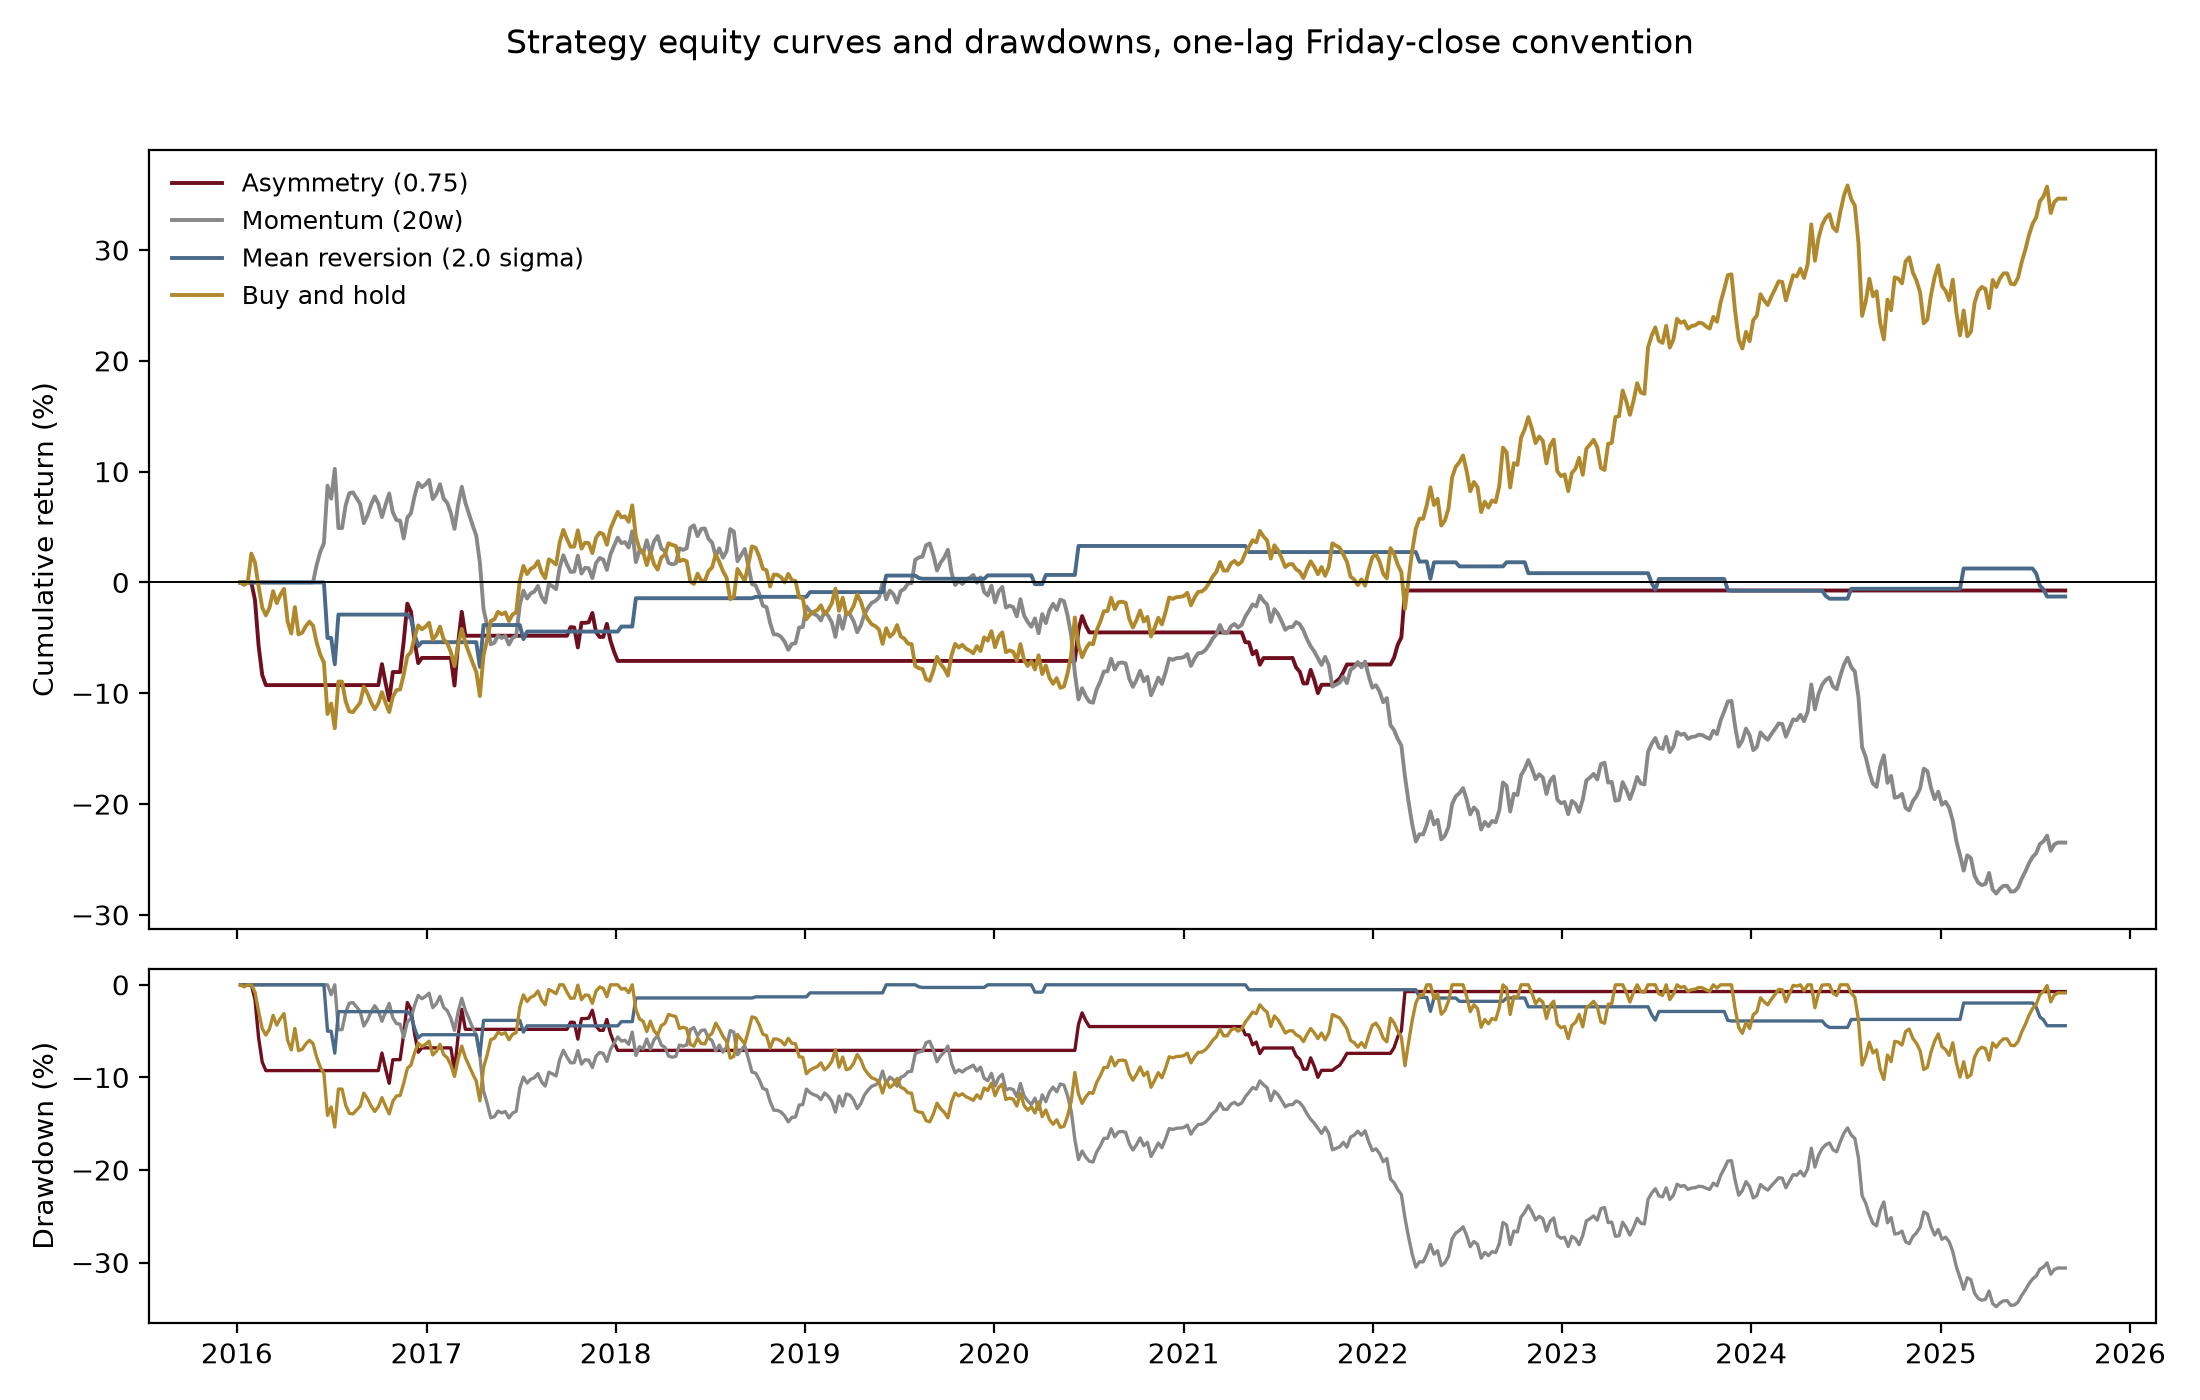
\includegraphics[width=\textwidth]{backtest_results.png}
\caption{Strategy equity curves and drawdowns (enlarged). Cumulative gross returns and drawdown profiles for the asymmetry strategy, the 20-week momentum and 2.0$\sigma$ mean-reversion benchmarks, and buy-and-hold on the 504-week EUR/JPY sample.}
\label{fig:backtest-enlarged}
\end{figure}

\end{document}
